\documentclass[twocolumn,10pt]{article}
\title{Area, volume, and surface area 2D and 3D objects }
\setlength{\columnsep}{20pt} 
\usepackage{amsmath,hyperref,cancel,graphicx}
 \def\shrinkfactor{0.4}
 \usepackage[margin=1.5cm]{geometry}
\usepackage[usenames,dvipsnames]{color}
 
 \newcommand{\blue}[1]{{\color{Blue}#1}} 
 \newcommand{\purple}[1]{{\color{Purple}#1}} 
 \newcommand{\red}[1]{{\color{Red}#1}} 
 \newcommand{\green}[1]{{\color{Green}#1}} 
 \newcommand{\gray}[1]{{\color{Gray}#1}} 
  \newcommand{\pink}[1]{{\color{Magenta}#1}}   



\begin{document}
\maketitle



\section{\href{https://www.khanacademy.org/devadmin/content/items/x06b1691221f6ea7d}{x06b1691221f6ea7d}}

\noindent
The Gangas are moving from Minneapolis to Mongolia. They pack their belongings in rectangular crates and hire a boxcar to ship the crates across land and sea.  Each crate has a base $10.1\text{ ft}$ long by $6\text{ ft}$ wide and height $10\text{ ft}$. The crates are made specifically to fit inside the boxcar. The boxcar is $50.5\text{ ft}$ long, $12\text{ ft}$ wide and $10\text{ ft}$ high. 

**How many crates can fit into one boxcar?**


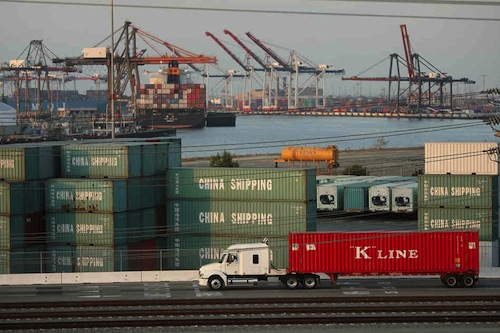
\includegraphics[scale=\shrinkfactor]{figures/203f27adba8bd870f05dc901ffbda2840eaf7d90.jpeg}

\paragraph{Ans} [[? input-number 1]] crates  10

\paragraph{Hint 1}Let's find the relationship between the lengths, widths and heights of the crate and the boxcar:

\begin{align*} 
10.1\text{ ft}\times5 &=50.5\text{ ft}  \\[2mm]
6\text{ ft}\times2      &=12\text{ ft}  \\[2mm]
10\text{ ft}\times1     &=10\text{ ft}
\end{align*}

\paragraph{Hint 2}Because the dimensions of the crate and boxcar are related, we can relate the volumes of the crate and boxcar in cubic feet. If we divide the volume of the boxcar by the volume of a crate, we can find how many crates The Gangas can fit into one boxcar.

The formula for volume $V$ of a rectangular prism is:

$\text{V} = \text{length}\cdot\text{width}\cdot\text{height}$

\paragraph{Hint 3}Let's find the volume of the boxcar in cubic feet:

\begin{align*} 
\blue{\text{V}_{\text{boxcar}}}
&= \text{length}\cdot\text{width}\cdot\text{height}\\[2mm]
&=50.5\times12\times10\\[2mm]
&=\blue{6060}\text{ ft}^3
\end{align*}

\paragraph{Hint 4}Let's find  the volume of one crate in cubic feet:

\begin{align*}
\pink{\text{V}_{\text{crate}}}
&= \text{length}\cdot\text{width}\cdot\text{height}\\[2mm]
&=10.1\times6\times10\\[2mm]
&=\pink{606}\text{ ft}^3
\end{align*}

\paragraph{Hint 5}To find how many crates fit in one boxcar, we can divide the volume of the boxcar by the volume of a crate: 

\begin{align*}
\dfrac{
  \blue{\text{V}_{\text{boxcar}}}
}{
  \pink{\text{V}_{\text{crate}}}
}
&=\dfrac{\blue{6060}}{\pink{606}}\\[1mm]
&=\ \green{10}\end{align*}

\paragraph{Hint 6}The Gangas can fit $\green{10}$ crates into one boxcar.



\medskip
\noindent
\textbf{Tags:} {\footnotesize Image needs attribution,  Area, volume, and surface area of 2d and 3d objects, CC.7.G.B.6}\\
\textbf{Version:} 8eb9ce46.. 2013-10-18
\smallskip\hrule





\section{\href{https://www.khanacademy.org/devadmin/content/items/x0dcefb4fdcbf8315}{x0dcefb4fdcbf8315}}

\noindent
Abuto plans to put in wall-to-wall carpet in his living room. He measures the edges of his living room and sketches up the following floor plan. The carpet costs $\$30$ per square meter. 

**How much will Abuto pay for wall-to-wall carpet for his entire living room?**   

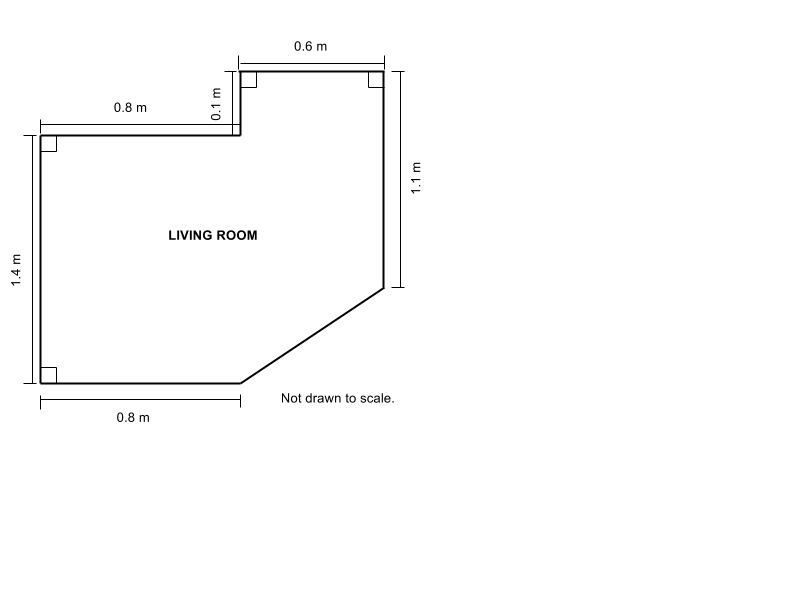
\includegraphics[scale=\shrinkfactor]{figures/9b1e5c4a0a1124465ed46125df08ae907b12b004.png}

\paragraph{Ans} $\$$ [[? input-number 1]]  57

\paragraph{Hint 1}Abuto's living room has $3$ rectangular areas and $1$ triangular area to cover with carpet. Let's find the total area of the living room floor in square meters to find how much carpet Abuto needs.

Area of a rectangle is equal to its length times its width. Area of a triangle is equal to one half its base times its height. 

\paragraph{Hint 2}From the vertical dimensions, we can determine the height of the triangle as $\red{0.4}\text{ m}$. We can also find the dimensions of the areas.
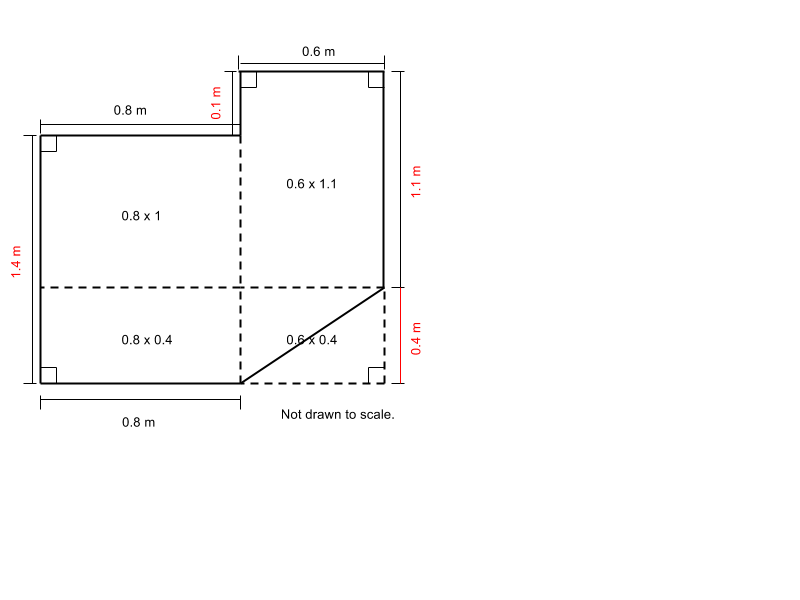
\includegraphics[scale=\shrinkfactor]{figures/58a4ba6e006a4cfc3f99cbaea0652a702b968dff.png}

\paragraph{Hint 3}Let's find the total area of the living room by adding the areas of the $3$ rectangles and $1$ triangle together. 

\begin{align*}  
\purple{\text{total area}} &= 0.8\times1  \ +\ 0.8\times 0.4\ +\ 0.6\times1.1 \ +\  \dfrac{1}{2}\times0.6\times\red{0.4}\\[2mm]
&=0.8+0.32+0.66+0.12\\[2mm]
&= \purple{1.9} \text{ m}^2
\end{align*}

\paragraph{Hint 4}Abuto has $\purple{1.9}\text{ m}^2$ to cover with carpet, and the cost of carpet is $\$\green{30}$ per square meter. Let's multiply the total area times the cost per area:

\begin{align*} 
\blue{\text{total cost}} &= \green{30}\times\purple{1.9}\\&=\$\blue{ 57}\end{align*}

\paragraph{Hint 5}Abuto will pay $\$\blue{57}$ to install wall-to-wall carpet in his living room.



\medskip
\noindent
\textbf{Tags:} {\footnotesize Images with English text,  Area, volume, and surface area of 2d and 3d objects, CC.7.G.B.6}\\
\textbf{Version:} 69a87b02.. 2013-10-18
\smallskip\hrule





\section{\href{https://www.khanacademy.org/devadmin/content/items/x0e6445ad25557e40}{x0e6445ad25557e40}}

\noindent
Tony plans to put in carpet in his living room. He measures the edges of his living room and sketches up the following floor plan. 

**How many square meters of carpet does Tony need to cover the entire area of his living room floor?**

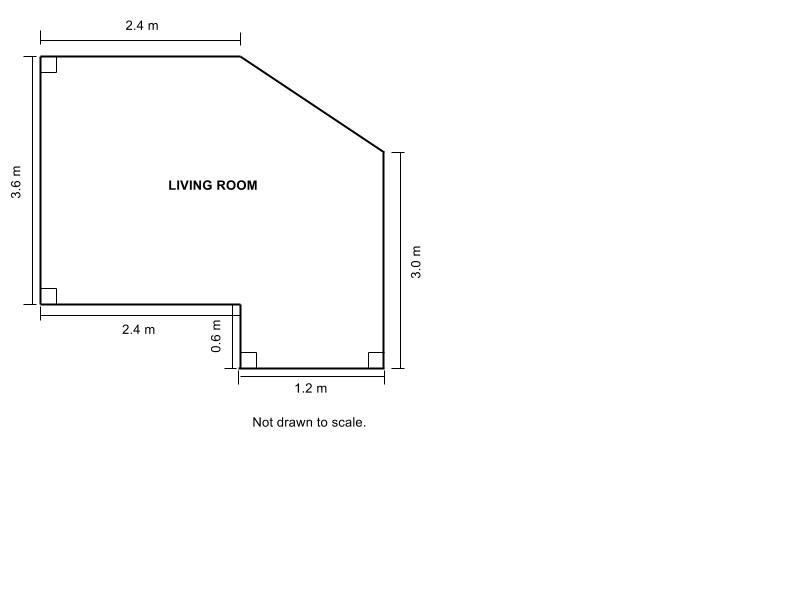
\includegraphics[scale=\shrinkfactor]{figures/046f049679d81a6e9e292791541c4b03dbcf7768.png}

\paragraph{Ans} [[? input-number 1]] $\text{m}^2$  12.96

\paragraph{Hint 1}Tony's living room has $3$ rectangular areas and $1$ triangular area to cover with carpet. Let's find the total area of the living room floor in square meters to find how much carpet Tony needs.

Area of a rectangle is equal to its length times its width. Area of a triangle is equal to one half its base times its height. 

\paragraph{Hint 2}From the vertical dimensions, we can determine the height of the triangle as $\red{1.2}$ m. We can also find the dimensions of the areas. 

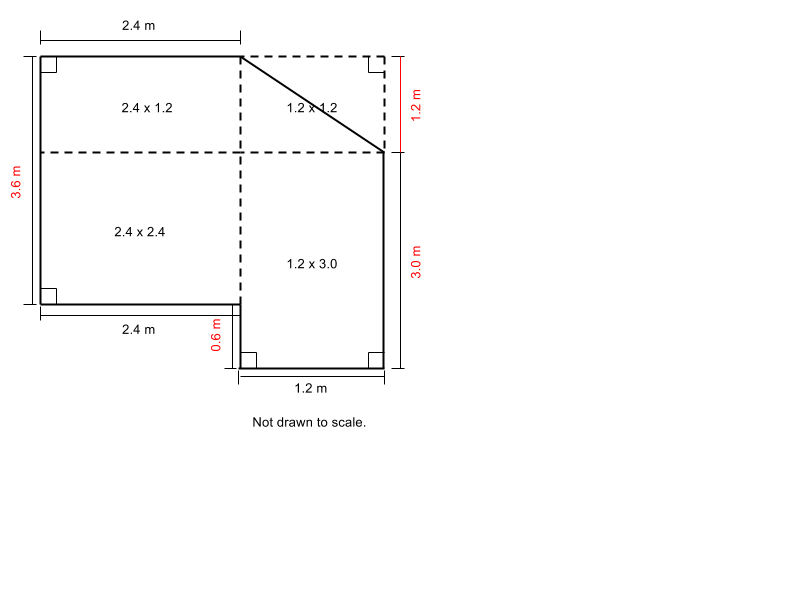
\includegraphics[scale=\shrinkfactor]{figures/bf7eaf5031a5e491d306dade1ef1176bfc6d4857.png}

\paragraph{Hint 3}Let's find the total area of the living room by adding the areas of the $3$ rectangles and $1$ triangle together. 

\begin{align*}  
&= 2.4\times1.2 +2.4^2+1.2\times3.0+ \frac{1}{2}\times1.2\times\red{1.2}\\\\&=2.88+5.76+3.6+0.72\\\\
&= \purple{12.96} \text{ m}^2\end{align*}

\paragraph{Hint 4}Tony needs $\purple{12.96}$ m$^2$ of carpet to cover the entire area of his living room floor.



\medskip
\noindent
\textbf{Tags:} {\footnotesize Images with English text,  Area, volume, and surface area of 2d and 3d objects, CC.7.G.B.6}\\
\textbf{Version:} 8ee1b817.. 2013-10-18
\smallskip\hrule





\section{\href{https://www.khanacademy.org/devadmin/content/items/x10eb0d14b6e1f311}{x10eb0d14b6e1f311}}

\noindent
The company Sweet as Pie has $500$ mile-high pumpkin pies to make for Thanksgiving. They package their pies each in a folded box made of cardboard. The closed box is a cube with side lengths $9\text{ in}$. There are $7$ rectangular tabs that wrap around the edges to make sure the pies stay fresh. The tabs are $9\text{ in}$ by $2\text{ in}$ each.

**In square inches what is the minimum amount of cardboard Sweet as Pie needs to package all $500$ pumpkin pies individually?**   

(Assume there is no wasted cardboard.)  

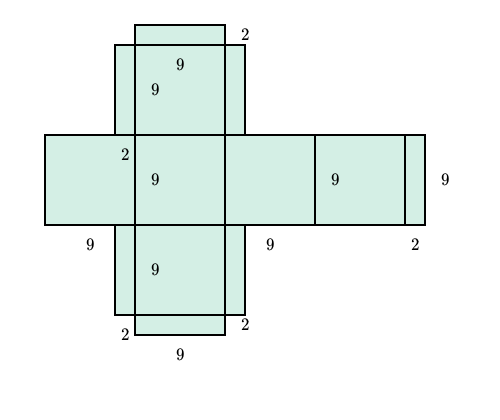
\includegraphics[scale=\shrinkfactor]{figures/9ee87af5745eecf3946aa60a923f2788c1dea2bf.png}

\paragraph{Ans} [[? input-number 1]] $\text{in}^2$  306000

\paragraph{Hint 1}Let's determine the surface area (SA) of one box in square inches. Then, we can multiply the surface area of one box times $\gray{500}$ to find how many square inches of cardboard are needed.

The box has is a cube, so it has $\green6$ square sides. The box also has $\purple7$ rectangular tabs.

\paragraph{Hint 2}Let's find the total surface area of the box. Area of a rectangle is equal to its length times its width. Let's find the surface areas of the $\green6$ square sides and $\purple7$ rectangular tabs.

There are $\green{6}$ square sides with side lengths $\blue{9}\text{ in}$:
 
\begin{align*} A_{\text{sides}} &= \green{6}\times\blue{9}\times\blue{9}\\
&= 486\text{ in}^2\end{align*}

There are $\purple7$ rectangular tabs $\blue{9}\text{ in}$ by $\pink{2}\text{ in}$:
 
\begin{align*} A_{\text{tabs}} &= \purple{7}\times\blue{9}\times\pink{2}\\
&= 126\text{ in}^2\end{align*}

Let�s sum together all the areas to find the total amount of cardboard required to make one box: 

\begin{align*} A_{\text{box}} 
&= A_{\text{sides}} +   A_{\text{tabs}} \\[2mm]
&= 486 + 126\\[2mm]
&= 612\text{ in}^2\end{align*}

\paragraph{Hint 3}The total amount of cardboard required to make $\gray{500}$ boxes is

\begin{align*} 
A_{\text{total}} &= \gray{500}\times612\\[2mm]
&= \red{306000}\text{ in}^2\end{align*}

\paragraph{Hint 4}Sweet as Pie needs a minimum of $\red{306,000}\text{ in}^2$ of cardboard to package all $\gray{500}$ pumpkin pies individually.



\medskip
\noindent
\textbf{Tags:} {\footnotesize Image needs attribution,  Area, volume, and surface area of 2d and 3d objects, CC.7.G.B.6}\\
\textbf{Version:} af91f822.. 2013-10-18
\smallskip\hrule





\section{\href{https://www.khanacademy.org/devadmin/content/items/x2303e1e7ce324859}{x2303e1e7ce324859}}

\noindent
Molly wants to know the volume of her gold ring in cubic centimeters. She gets a glass in the shape of rectangular prism with a base $3\text{ cm}$ by $2\text{ cm}$ and fills the glass with $3.1\text{ cm}$ of water. Molly drops her gold ring in the glass and measures the new height of the water to be $3.7\text{ cm}$. 

**What is the volume of Molly's ring in cubic centimeters?**



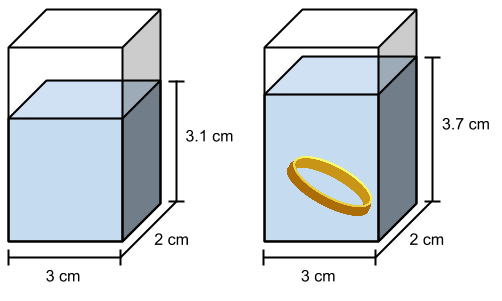
\includegraphics[scale=\shrinkfactor]{figures/6a170f3839757fae9ea33580d7e13567cc0e63e8.png}

\paragraph{Ans} [[? input-number 1]] $\text{cm}^3$  3.6

\paragraph{Hint 1}The change in volume of the water is caused by adding the volume of Molly's gold ring to the volume of the water. Let's find the change in volume to find the volume of the gold ring.

Volume $V$ of a rectangular prism can be calculated using the formula:

$\text{V} = \text{length}\cdot\text{width}\cdot\text{height}$

\paragraph{Hint 2}The length $\green3\text{ cm}$ and width $\purple2\text{ cm}$ of the water in the rectangular glass does not change, only the height of the water changes. 

\paragraph{Hint 3}The change in height of the water is $\blue{(3.7-3.1)}\text{ cm}$. Let's find $V$ of the change in water:

\begin{align*} V_{\text{ring}} &= \text{length}\cdot\text{width}\cdot(\text{change in height})\\
&= \green3\cdot\purple2\cdot\blue{(3.7-3.1)}\\&= \green3\cdot\purple2\cdot\blue{(0.6)}\\
&= \red{3.6}\text{ cm}^3\end{align*}

\paragraph{Hint 4}The volume of Molly's gold ring is $\red{3.6}\text{ cm}^3$.



\medskip
\noindent
\textbf{Tags:} {\footnotesize Image needs attribution,  Area, volume, and surface area of 2d and 3d objects, CC.7.G.B.6}\\
\textbf{Version:} 20d2bf89.. 2013-10-18
\smallskip\hrule





\section{\href{https://www.khanacademy.org/devadmin/content/items/x23beb4cd843665af}{x23beb4cd843665af}}

\noindent
The Joneses are moving from San Francisco to South Africa. They pack their belongings in rectangular crates and hire a boxcar to ship the crates across land and sea.  The crates are made specifically to fit inside the boxcar with their bases facing down. Each crate has a base $15\text{ ft}$ long by $5\text{ ft}$ wide and height $6.5\text{ ft}$. The boxcar is $60\text{ ft}$ long, $10\text{ ft}$ wide and $13\text{ ft}$ high. 

**How many crates can The Joneses fit into one boxcar?**


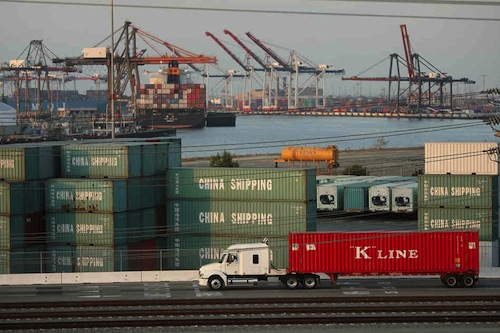
\includegraphics[scale=\shrinkfactor]{figures/203f27adba8bd870f05dc901ffbda2840eaf7d90.jpeg}

\paragraph{Ans} [[? input-number 1]] crates  16

\paragraph{Hint 1}Let's find the relationship between the lengths, widths and heights of the crate and boxcar:

\begin{align*} 15\text{ ft}\times4&=60\text{ ft}\\\\5\text{ ft}\times2&=10\text{ ft}\\\\6.5\text{ ft}\times2&=13\text{ ft}\end{align*}

\paragraph{Hint 2}Because the dimensions of the crate and boxcar are related, we can relate the volumes of the crate and boxcar in cubic feet. If we divide the volume of the boxcar by the volume of a crate, we can find how many crates The Joneses can fit into one boxcar.

The formula for volume $V$ of a rectangular prism is:

$\text{V} = \text{length}\cdot\text{width}\cdot\text{height}$

\paragraph{Hint 3}Let's find  $V$ of the boxcar in cubic feet:

\begin{align*} \text{V} &= \text{length}\cdot\text{width}\cdot\text{height}\\&=60\times10\times13\\&=\blue{7800}\text{ ft}^3\end{align*}

\paragraph{Hint 4}Let's find  $V$ of a crate in cubic feet:

\begin{align*} \text{V} &= \text{length}\cdot\text{width}\cdot\text{height}\\&=15\times5\times6.5\\&=\pink{487.5}\text{ ft}^3\end{align*}

\paragraph{Hint 5}Now, let's divide the volume of the boxcar by the volume of a crate to find how many crates:

\begin{align*}\ &=\blue{7800}\div\pink{487.5}\\&=\green{16}\end{align*}

\paragraph{Hint 6}The Joneses can fit $\green{16}$ crates into one boxcar.



\medskip
\noindent
\textbf{Tags:} {\footnotesize Image needs attribution,  Area, volume, and surface area of 2d and 3d objects, CC.7.G.B.6}\\
\textbf{Version:} af6cf468.. 2013-10-14
\smallskip\hrule





\section{\href{https://www.khanacademy.org/devadmin/content/items/x276127b5872fbc61}{x276127b5872fbc61}}

\noindent
The company Sweet as Pie has $750$ mile-high apple pies to make for Thanksgiving. They package their pies each in a folded box made out of cardboard. The closed box is a cube with side lengths $8\text{ in}$. There are $7$ rectangular tabs that wrap around the edges to make sure the pies stay fresh. The tabs are $8\text{ in}$ by $2\text{ in}$ each.

**In square inches what is the minimum amount of cardboard Sweet as Pie needs to package all $750$ apple pies individually? (Assume there is no wasted cardboard.)**


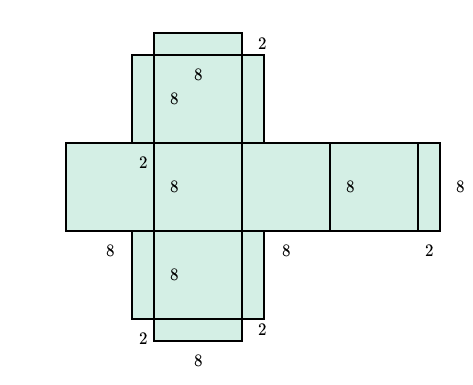
\includegraphics[scale=\shrinkfactor]{figures/a118c7f7a06b93f92f4dfa5551cf739f2755885d.png}

\paragraph{Ans} [[? input-number 1]] $\text{in}^2$  650000

\paragraph{Hint 1}Let�s determine the surface area (SA) of one box in square inches. Then, we can multiply the surface area of one box times $\gray{750}$ to find how many square inches of cardboard are needed.

The box has is a cube, so it has $\green6$ square sides. The box also has $\purple7$ rectangular tabs.

\paragraph{Hint 2}Let�s find the total surface area of the box. Area of a rectangle is equal to its length times its width. Let's find the surface areas of the $\green6$ square sides and $\purple7$ rectangular tabs.

There are $\green{6}$ square sides with side lengths $\blue{8}\text{ in}$:
 
\begin{align*} SA &= \green{6}\times\blue{8}\times\blue{8}\\
&= 384\text{ in}^2\end{align*}

There are $\purple7$ rectangular tabs $\blue{8}\text{ in}$ by $\pink{2}\text{ in}$:
 
\begin{align*} SA &= \purple{7}\times\blue{8}\times\pink{2}\\
&= 112\text{ in}^2\end{align*}

Let�s sum together all the surface areas to find the total surface area of one box: 

\begin{align*} SA &= 384 + 112\\
&= 496\text{ in}^2\end{align*}

\paragraph{Hint 3}Let's multiply the total area by $\gray{750}$ boxes to find the amount of cardboard:

\begin{align*} SA &= \gray{750}\times496\\&= \red{372000}\text{ in}^2\end{align*}

\paragraph{Hint 4}Sweet as Pie needs a minimum of $\red{372,000}\text{ in}^2$ of cardboard to package all $\gray{750}$ apple pies individually.



\medskip
\noindent
\textbf{Tags:} {\footnotesize Image needs attribution,  Area, volume, and surface area of 2d and 3d objects, CC.7.G.B.6}\\
\textbf{Version:} d70f2a95.. 2013-10-14
\smallskip\hrule





\section{\href{https://www.khanacademy.org/devadmin/content/items/x27952dc36dd03124}{x27952dc36dd03124}}

\noindent
A crew is excavating a construction site to build a new swimming pool. The crew fills the box of a dump truck to the top with earth. The box is $40\text{ ft}$ long, $25\text{ ft}$ wide, and $20\text{ ft}$ high. In transport to the dump site, the volume of the earth decreases by $15\%$ as it settles in the box. 

**What is the volume of the soil when it reaches the dump site?**


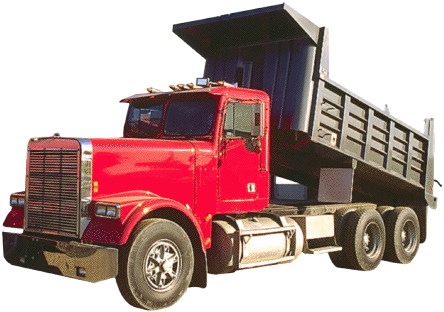
\includegraphics[scale=\shrinkfactor]{figures/e5db961622b94a55a7cbe0a2b2c1a6c7_AdPanel.png}

\paragraph{Ans} [[? input-number 1]] $\text{ft}^3$  17000

\paragraph{Hint 1}The length and width of the soil in the box of the truck does not change, but the height of the soil changes. The height of the soil decreases by $15\%$ during the transport.

The soil is $\green{85}\%$ of its original height when it reaches the dump, since $100\%-15\%=\green{85}\%$.



\paragraph{Hint 2}Let's multiply the original height $\purple{20}\text{ ft}$ by $\green{0.85}$  to find the height of the soil at the dump site:

\begin{align*} \pink{\text{height}} &= \green{0.85}\cdot\purple{20}\\&= \pink{17}\text{ ft}\end{align*}

\paragraph{Hint 3}Now, let's find the volume of the soil using the formula for volume $V$ of a rectangular prism and the dimensions of the soil at the dump site:

\begin{align*} \blue{V} &= \text{length}\cdot\text{width}\cdot\text{height}\\[2mm]
&= 40\cdot25\cdot\pink{17}\\[2mm]
&= \blue{17000}\text{ ft}^3
\end{align*}

\paragraph{Hint 4}The volume of soil when it reaches the dump site is $\blue{17,000}\text{ ft}^3$.



\medskip
\noindent
\textbf{Tags:} {\footnotesize Image needs attribution,  Area, volume, and surface area of 2d and 3d objects, CC.7.G.B.6}\\
\textbf{Version:} 5146f38b.. 2013-10-18
\smallskip\hrule





\section{\href{https://www.khanacademy.org/devadmin/content/items/x27ff33d9c309c7ce}{x27ff33d9c309c7ce}}

\noindent
A crew is excavating a construction site to build a new swimming pool. The crew fills the box of a dump truck to the top with dirt. The box is $40\text{ ft}$ long, $35\text{ ft}$ wide, and $30\text{ ft}$ high. In transport to the dump site, the volume of the soil decreases $20\%$ as it settles in the box. 

**What is the height in feet of the dirt at the dump site?**




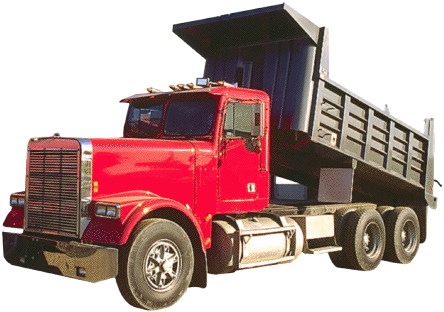
\includegraphics[scale=\shrinkfactor]{figures/e5db961622b94a55a7cbe0a2b2c1a6c7_AdPanel.png}

\paragraph{Ans} [[? input-number 1]] $\text{ft}$  24

\paragraph{Hint 1}The length and width of the soil in the box does not change, but the height does change. Only the height of the soil decreases $20\%$. So, the soil is $\green{80}\%$ of its original height.



\paragraph{Hint 2}Let's multiply the height $\purple{30}\text{ ft}$ by $\green{0.8}$  to find the height of the soil at the dump site:

\begin{align*} h &= \green{0.8}\cdot\purple{30}\\&= \pink{24}\text{ ft}\end{align*}

\paragraph{Hint 3}The soil is $\pink{24}\text{ ft}$ at the dump site.



\medskip
\noindent
\textbf{Tags:} {\footnotesize Image needs attribution,  Area, volume, and surface area of 2d and 3d objects, CC.7.G.B.6}\\
\textbf{Version:} 72a8546b.. 2013-10-14
\smallskip\hrule





\section{\href{https://www.khanacademy.org/devadmin/content/items/x2d596dc8eec89b08}{x2d596dc8eec89b08}}

\noindent
The company Digit Tech designs a new SmartPhone. The packaging includes an open box made out of cardboard. The dimensions of the box are $15\text{ cm}$ long, $10\text{ cm}$  wide and $10\text{ cm}$  high. Digit Tech expects to sell $1000$ phones and package each phone individually in a box. 

**In square centimeters what is the minimum amount of cardboard Digit Tech needs to package all $1000$ new SmartPhones? (Assume there is no wasted cardboard.)**


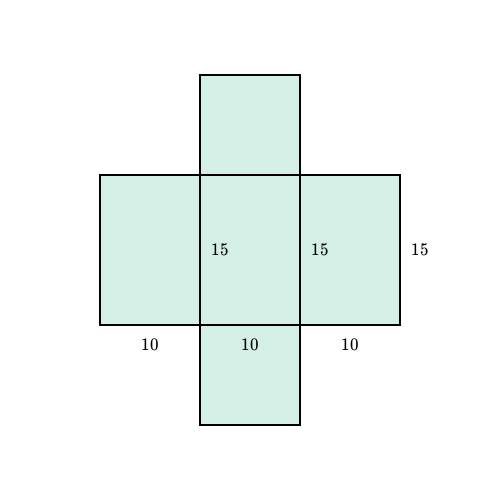
\includegraphics[scale=\shrinkfactor]{figures/69a70b16cec3997bfa665a611382451946b7bf54.png}

\paragraph{Ans} [[? input-number 1]] $\text{cm}^2$  650000

\paragraph{Hint 1}Let�s determine the surface area (SA) of one box in square centimeters. Then, we can multiply the surface area of one box times $\purple{1000}$ to find how many square centimeters of cardboard are needed.

The box has $5$ sides: $1$ bottom and $2$ sets of equal sides opposite each other.

\paragraph{Hint 2}Let�s find the total surface area of the box. Area of a rectangle is equal to its length times its width. Let's find the surface areas of the $5$ rectangular sides.

There are $\gray{2}$ sides $\blue{15}\text{ cm}$ long and $\green{10}\text{ cm}$ high:
 
\begin{align*} SA &= \gray{2}\times\blue{15}\times\green{10}\\
&= 300\text{ cm}^2\end{align*}

There are $\gray{2}$ sides $\pink{10}\text{ cm}$ wide and $\green{10}\text{ cm}$ high:
 
\begin{align*} SA &= \gray{2}\times\pink{10}\times\green{10}\\
&= 200\text{ cm}^2\end{align*}

There is $\gray{1}$ side (the bottom) $\blue{15}$ cm long and $\pink{10}$ cm wide:

\begin{align*} SA &= \gray{1}\times\blue{15}\times\pink{10}\\
&= 150\text{ cm}^2\end{align*}

Let�s sum together all the surface areas to find the total surface area of one box: 

\begin{align*} SA &= 300 + 200 + 150\\
&= 650\text{ cm}^2\end{align*}

\paragraph{Hint 3}Let's multiply the total area by $\purple{1000}$ boxes to find the amount of cardboard:

\begin{align*} SA &= \purple{1000}\times650\\&= \pink{650000}\text{ cm}^2\end{align*}

\paragraph{Hint 4}Digit Tech needs a minimum of $\pink{650,000}\text{ cm}^2$ of cardboard to package all $\purple{1000}$ new SmartPhones individually.



\medskip
\noindent
\textbf{Tags:} {\footnotesize Image needs attribution,  Area, volume, and surface area of 2d and 3d objects, CC.7.G.B.6}\\
\textbf{Version:} 207d6a6d.. 2013-10-14
\smallskip\hrule





\section{\href{https://www.khanacademy.org/devadmin/content/items/x33396169090e3680}{x33396169090e3680}}

\noindent
The Smiths are moving from New York to Shanghai. They pack their belongings in rectangular crates and hire a boxcar to ship the crates across land and sea.  The crates are made specifically to fit inside the boxcar with their bases facing down. Each crate has a base $10\text{ ft}$ long by $4.5\text{ ft}$ wide and height $6\text{ ft}$. The boxcar is $50\text{ ft}$ long, $9\text{ ft}$ wide and $12\text{ ft}$ high. 

**How many crates can The Smiths fit into one boxcar?**


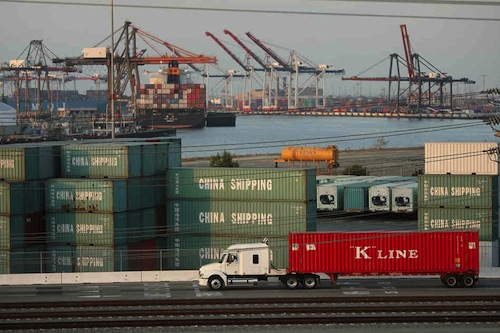
\includegraphics[scale=\shrinkfactor]{figures/203f27adba8bd870f05dc901ffbda2840eaf7d90.jpeg}

\paragraph{Ans} [[? input-number 1]] crates  20

\paragraph{Hint 1}Let's find the relationship between the lengths, widths and heights of the crate and boxcar:

\begin{align*} 10\text{ ft}\times5&=50\text{ ft}\\\\4.5\text{ ft}\times2&=9\text{ ft}\\\\6\text{ ft}\times2&=12\text{ ft}\end{align*}

\paragraph{Hint 2}Because the dimensions of the crate and boxcar are related, we can relate the volumes of the crate and boxcar in cubic feet. If we divide the volume of the boxcar by the volume of a crate, we can find how many crates The Smiths can fit into one boxcar.

The formula for volume $V$ of a rectangular prism is:

$\text{V} = \text{length}\cdot\text{width}\cdot\text{height}$

\paragraph{Hint 3}Let's find  $V$ of the boxcar in cubic feet:

\begin{align*} \text{V} &= \text{length}\cdot\text{width}\cdot\text{height}\\&=50\times9\times12\\&=\blue{5400}\text{ ft}^3\end{align*}

\paragraph{Hint 4}Let's find  $V$ of a crate in cubic feet:

\begin{align*} \text{V} &= \text{length}\cdot\text{width}\cdot\text{height}\\&=10\times4.5\times6\\&=\pink{270}\text{ ft}^3\end{align*}

\paragraph{Hint 5}Now, let's divide the volume of the boxcar by the volume of a crate to find how many crates:

\begin{align*}\ &=\blue{5400}\div\pink{270}\\&=\green{20}\end{align*}

\paragraph{Hint 6}The Smiths can fit $\green{20}$ crates into one boxcar.



\medskip
\noindent
\textbf{Tags:} {\footnotesize Image needs attribution,  Area, volume, and surface area of 2d and 3d objects, CC.7.G.B.6}\\
\textbf{Version:} 39d1acc8.. 2013-10-14
\smallskip\hrule





\section{\href{https://www.khanacademy.org/devadmin/content/items/x3e93af40b7f72c90}{x3e93af40b7f72c90}}

\noindent
Molly made each of her $12$ girlfriends a pair of earrings. To wrap the pairs individually, she creates a simple cardboard gift box to fold into a pyramid. The base is a square with side lengths $10\text{ in}$. The sides are $4$ equilateral triangles with side lengths $10\text{ in}$ and height $h$. The height $h$ is equal to $8\!\frac{2}{3}\text{ in}$. 

**In square inches what is the minimum amount of cardboard Molly needs to create $12$ gift boxes to wrap each pair of earrings individually? (Assume there is no wasted cardboard.)**


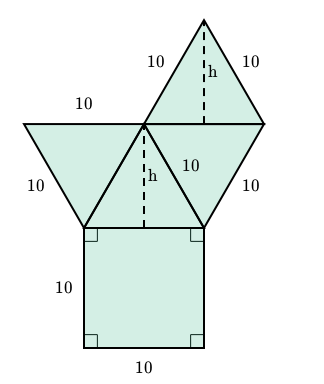
\includegraphics[scale=\shrinkfactor]{figures/9b1a8c58e358c5d122dd18071886f4cdf8867b8f.png} 

\paragraph{Ans} [[? input-number 1]] $\text{in}^2$  3280

\paragraph{Hint 1}Let�s determine the surface area (SA) of one box in square inches. Then, we can multiply the surface area of one box times $\gray{12}$ to find how many square inches of cardboard are needed. 

Let's use fractions throughout our calculations to avoid any rounding errors.

\paragraph{Hint 2}Let�s find the total surface area of the box by finding the surface areas of $1$ square and $\purple4$ triangles.

 Area of a square is equal to its length squared. There is $1$ square side with side lengths $\blue{10}\text{ in}$:
 
\begin{align*} SA &= \blue{10}^2\\
&= 100\text{ in}^2\end{align*}

Area of a triangle is equal to one half its base times its height $h$. There are $\purple4$ triangles with a base of $\blue{10}\text{ in}$ and height of $\pink{8\frac{2}{3}}\text{ in}$:
 
\begin{align*} SA &= \purple{4}\times\dfrac{1}{2}\times\blue{10}\times\pink{8\dfrac{2}{3}}\\\\&=\purple{4}\times\blue{10}\times\dfrac{1}{2}\times\pink{\dfrac{26}{3}}\\\\
&= \dfrac{1040}{6}\\\\&= \dfrac{520}{3}\text{ in}^2\end{align*}

Let�s sum together all the surface areas to find the total surface area of one box: 

\begin{align*} SA &= 100 +  \dfrac{520}{3}\\\\&= \dfrac{300}{3}+ \dfrac{520}{3}\\\\
&=  \dfrac{820}{3}\text{ in}^2\end{align*}

\paragraph{Hint 3}Let's multiply the total area by $\gray{12}$ boxes to find the amount of cardboard:

\begin{align*} SA &= \gray{12}\times \dfrac{820}{3}\\&= \red{3280}\text{ in}^2\end{align*}

\paragraph{Hint 4}Molly needs a minimum of $\red{3280}\text{ in}^2$ of cardboard to package all $\gray{12}$ pairs of earrings individually.



\medskip
\noindent
\textbf{Tags:} {\footnotesize Image needs attribution,  Area, volume, and surface area of 2d and 3d objects, CC.7.G.B.6}\\
\textbf{Version:} 4aa17e10.. 2013-10-18
\smallskip\hrule





\section{\href{https://www.khanacademy.org/devadmin/content/items/x4e644b9868f4e7bb}{x4e644b9868f4e7bb}}

\noindent
Eric plans to put in carpet in his living room. He measures the edges of his living room and sketches up the following floor plan. 

**How many square feet of carpet does Eric need to cover the entire area of his living room floor?**

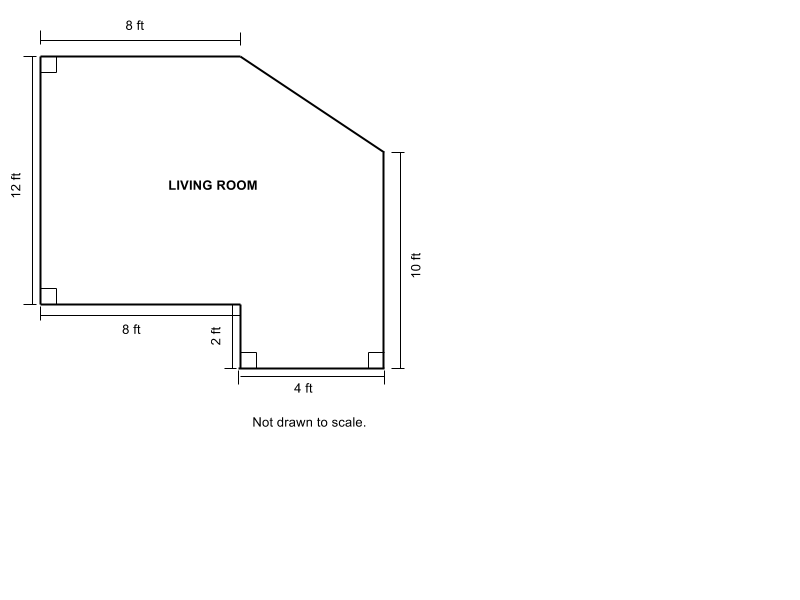
\includegraphics[scale=\shrinkfactor]{figures/3acac9e0deb063daeeca4749bfd6c9dbd2289ce2.png}

\paragraph{Ans} [[? input-number 1]] $\text{ft}^2$  144

\paragraph{Hint 1}Eric's living room has $3$ rectangular areas and $1$ triangular area to cover with carpet. Let's find the total area of the living room floor in square feet to find how much carpet Eric needs.

Area of a rectangle is equal to its length times its width. Area of a triangle is equal to one half its base times its height. 

\paragraph{Hint 2}From the vertical dimensions, we can determine the height of the triangle as $\red{4}$ ft. We can also find the dimensions of the areas. 

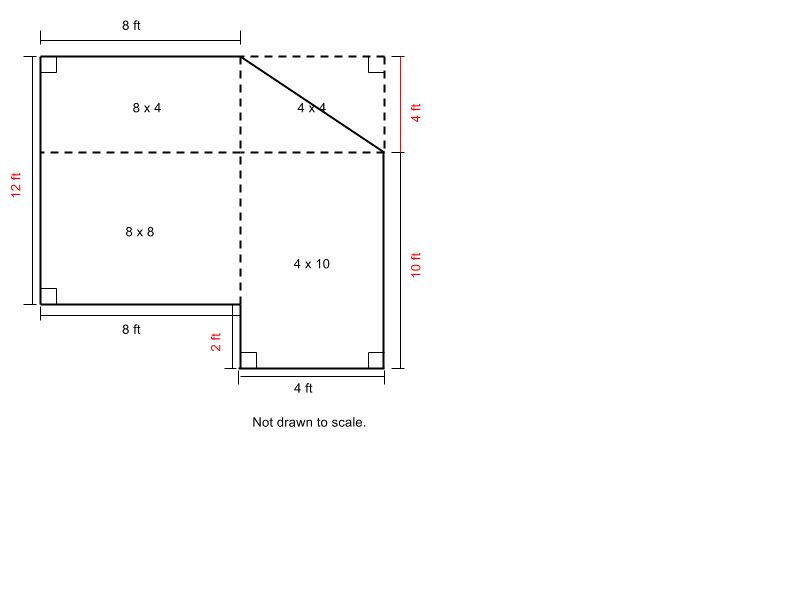
\includegraphics[scale=\shrinkfactor]{figures/809320a51fcfe278f60fb9dff4257df10294d43d.png}

\paragraph{Hint 3}Let's find the total area of the living room by adding the areas of the $3$ rectangles and $1$ triangle together. 

\begin{align*}  
&= 8\times4 +8^2+4\times10+ \dfrac{1}{2}\times4\times\red4\\\\&=32+64+40+8\\\\
&= \purple{144} \text{ ft}^2\end{align*}

\paragraph{Hint 4}Eric needs $\purple{144}$ ft$^2$ of carpet to cover the entire area of his living room floor.



\medskip
\noindent
\textbf{Tags:} {\footnotesize Images with English text,  Area, volume, and surface area of 2d and 3d objects, CC.7.G.B.6}\\
\textbf{Version:} 17ad5acd.. 2013-10-11
\smallskip\hrule





\section{\href{https://www.khanacademy.org/devadmin/content/items/x5482354a69951a95}{x5482354a69951a95}}

\noindent
A crew is excavating a construction site to build a new swimming pool. The crew fills the box of a dump truck to the top with dirt. The box is $13\text{ m}$ long, $10\text{ m}$ wide, and $10\text{ m}$ high. In transport to the dump site, the volume of the soil decreases $12\%$ as it settles in the box. 

**What is the volume of the dirt at the dump site in cubic meters?**




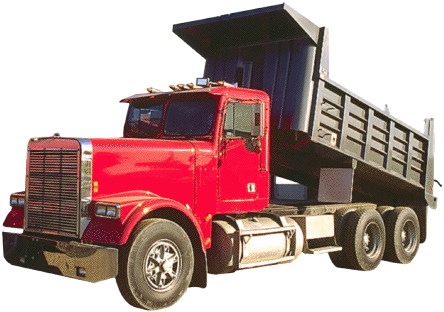
\includegraphics[scale=\shrinkfactor]{figures/e5db961622b94a55a7cbe0a2b2c1a6c7_AdPanel.png}

\paragraph{Ans} [[? input-number 1]] $\text{m}^3$  1144

\paragraph{Hint 1}The length and width of the soil in the box does not change, but the height does change. Only the height of the soil decreases $12\%$. 

In other words, the soil is $\green{88}\%$ of its original height at the dump site, since $100\%-12\%=\green{88}\%$.



\paragraph{Hint 2}Let's multiply the original height $\purple{10}\text{ m}$ by $\green{0.88}$  to find the height of the soil at the dump site:

\begin{align*} h &= \green{0.88}\cdot\purple{10}\\&= \pink{8.8}\text{ m}\end{align*}

\paragraph{Hint 3}Now, let's find the volume of the box using the formula for volume $\text{V}$ of a rectangular prism and the dimensions of the soil at the dump site:

\begin{align*} \text{V} &= \text{length}\cdot\text{width}\cdot\text{height}\\
&= 13\cdot10\cdot\pink{8.8}\\
&= \blue{1144}\text{ m}^3\end{align*}

\paragraph{Hint 4}The volume of the dirt at the dump site is $\blue{1144}\text{ m}^3$.



\medskip
\noindent
\textbf{Tags:} {\footnotesize Image needs attribution,  Area, volume, and surface area of 2d and 3d objects, CC.7.G.B.6}\\
\textbf{Version:} 72648da6.. 2013-10-14
\smallskip\hrule





\section{\href{https://www.khanacademy.org/devadmin/content/items/x63b88eeb5015ba3c}{x63b88eeb5015ba3c}}

\noindent
Jose is making a crazy math construction. He creates $360$ small pyramids out of paper he folds, then glues together identical sides until he makes a large pyramid. One small pyramid contains a square base with side lengths $a$ and $4$ equilateral triangles with base $a$ and height $h$. The height $h$ is $1.7\text{ cm}$. The length $a$ is $2\text{ cm}$. 

**In square centimeters what is the minimum amount of paper Jose uses to create $360$ small pyramids? (Assume there is no wasted paper.)**


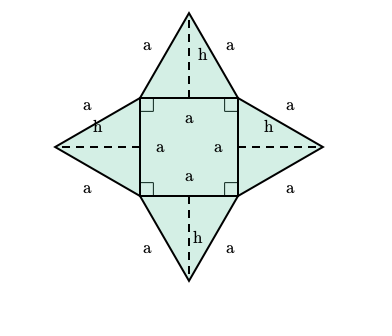
\includegraphics[scale=\shrinkfactor]{figures/6c9db7e28a2e7a3f87f8691e8eff1b044f8acbfd.png}

\paragraph{Ans} [[? input-number 1]] $\text{cm}^2$  3888

\paragraph{Hint 1}Let�s determine the surface area (SA) of one small pyramid in square centimeters. Then, we can multiply the surface area of one small pyramid times $\gray{360}$ to find how many square centimeters of paper Jose needs.

\paragraph{Hint 2}Let�s find the total surface area of a small pyramaid by finding the surface areas of $1$ square and $\purple4$ triangles.

 Area of a square is equal to its length squared. There is $1$ square side with side lengths $\blue{2}\text{ cm}$:
 
\begin{align*} SA &= \blue{2}^2\\
&= 4\text{ cm}^2\end{align*}

Area of a triangle is equal to one half its base times its height $h$. There are $\purple4$ triangles with a base of $\blue{2}$ and height of $\pink{1.7}\text{ cm}$:
 
\begin{align*} SA &= \purple{4}\times\dfrac{1}{2}\times\blue{2}\times\pink{1.7}\\
&= 6.8\text{ cm}^2\end{align*}

Let�s sum together all the surface areas to find the total surface area of one box: 

\begin{align*} SA &=4 + 6.8\\
&=  10.8\text{ cm}^2\end{align*}

\paragraph{Hint 3}Let's multiply the total area by $\gray{360}$ to find the amount of paper Jose needs:

\begin{align*} SA &= \gray{360}\times10.8\\&= \red{3888}\text{ cm}^2\end{align*}

\paragraph{Hint 4}Jose needs a minimum of $\red{3888}\text{ cm}^2$ of paper to create $\gray{360}$ small pyramids.



\medskip
\noindent
\textbf{Tags:} {\footnotesize Image needs attribution,  Area, volume, and surface area of 2d and 3d objects, CC.7.G.B.6}\\
\textbf{Version:} 925df6e3.. 2013-10-14
\smallskip\hrule





\section{\href{https://www.khanacademy.org/devadmin/content/items/x6648cea11832855f}{x6648cea11832855f}}

\noindent
A crew is excavating a construction site to build a new swimming pool. The crew fills the box of a dump truck to the top with dirt. The box is $12\text{ m}$ long, $10\text{ m}$ wide, and $10\text{ m}$ high. In transport to the dump site, the volume of the soil decreases $10\%$ as it settles in the box. 

**What is the volume of the dirt at the dump site in cubic meters?**




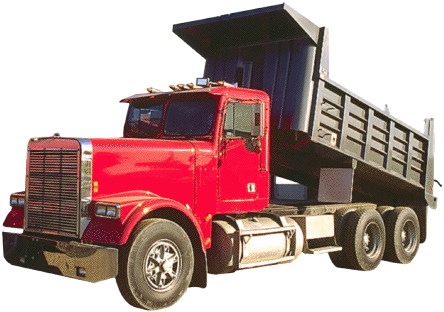
\includegraphics[scale=\shrinkfactor]{figures/e5db961622b94a55a7cbe0a2b2c1a6c7_AdPanel.png}

\paragraph{Ans} [[? input-number 1]] $\text{m}^3$  1080

\paragraph{Hint 1}The length and width of the soil in the box does not change, but the height does change. Only the height of the soil decreases $10\%$. 

In other words, the soil is $\green{90}\%$ of its original height at the dump site, since $100\%-12\%=\green{90}\%$.



\paragraph{Hint 2}Let's multiply the original height $\purple{10}\text{ m}$ by $\green{0.9}$  to find the height of the soil at the dump site:

\begin{align*} h &= \green{0.9}\cdot\purple{10}\\&= \pink{9}\text{ m}\end{align*}

\paragraph{Hint 3}Now, let's find the volume of the box using the formula for volume $\text{V}$ of a rectangular prism and the dimensions of the soil at the dump site:

\begin{align*} \text{V} &= \text{length}\cdot\text{width}\cdot\text{height}\\
&= 12\cdot10\cdot\pink{9}\\
&= \blue{1080}\text{ m}^3\end{align*}

\paragraph{Hint 4}The volume of the dirt at the dump site is $\blue{1080}\text{ m}^3$.



\medskip
\noindent
\textbf{Tags:} {\footnotesize Image needs attribution,  Area, volume, and surface area of 2d and 3d objects, CC.7.G.B.6}\\
\textbf{Version:} f00d0545.. 2013-10-14
\smallskip\hrule





\section{\href{https://www.khanacademy.org/devadmin/content/items/x6ed17026d8bfe0bb}{x6ed17026d8bfe0bb}}

\noindent
Laura wants to know the volume of her gold ring in cubic inches. She gets a rectangular glass with a base $3\text{ in}$ by $2\text{ in}$ and fills the glass $3.5\text{ in}$ high with water. Laura drops her gold ring in the glass and measures the new height of the water to be $3.8\text{ in}$. 

**What is the volume of Laura's ring in cubic inches?**


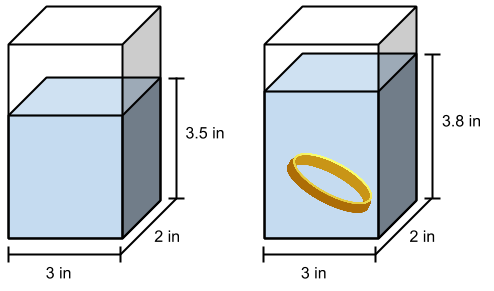
\includegraphics[scale=\shrinkfactor]{figures/4b9d2e0994214f17fec92b441910951b128b26b4.png}

\paragraph{Ans} [[? input-number 1]] $\text{in}^3$  1.8

\paragraph{Hint 1}The change in volume of the water is caused by adding the volume of Laura's gold ring to the volume of the water. Let's find the change in volume to find the volume of the gold ring.

Volume $V$ of a rectangular prism can be calculated using the formula:

$\text{V} = \text{length}\cdot\text{width}\cdot\text{height}$

\paragraph{Hint 2}The length $\green3\text{ in}$ and width $\purple2\text{ in}$ of the water in the rectangular glass does not change, but the height does change. 

\paragraph{Hint 3}The change in height of the water is $\blue{(3.8-3.5)}\text{ in}$. Let's find $V$ of the change in water:

\begin{align*} \text{V} &= \text{length}\cdot\text{width}\cdot\text{height}\\
&= \green3\cdot\purple2\cdot\blue{(3.8-3.5)}\\&= \green3\cdot\purple2\cdot\blue{(0.3)}\\
&= \red{1.8}\text{ in}^3\end{align*}

\paragraph{Hint 4}The volume of Laura's gold ring is $\red{1.8}\text{ in}^3$.



\medskip
\noindent
\textbf{Tags:} {\footnotesize Image needs attribution,  Area, volume, and surface area of 2d and 3d objects, CC.7.G.B.6}\\
\textbf{Version:} 40c1d84c.. 2013-10-14
\smallskip\hrule





\section{\href{https://www.khanacademy.org/devadmin/content/items/x7624e1cba96b8577}{x7624e1cba96b8577}}

\noindent
A crew is excavating a construction site to build a new swimming pool. The crew fills the box of a dump truck to the top with dirt. The box is $48\text{ ft}$ long, $24\text{ ft}$ wide, and $24\text{ ft}$ high. In transport to the dump site, the volume of the soil decreases $25\%$ as it settles in the box. 

**What is the height in feet of the dirt at the dump site?**



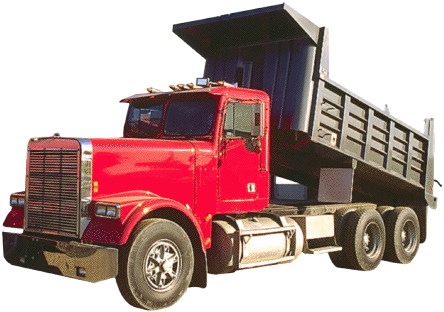
\includegraphics[scale=\shrinkfactor]{figures/e5db961622b94a55a7cbe0a2b2c1a6c7_AdPanel.png}

\paragraph{Ans} [[? input-number 1]] $\text{ft}$  18

\paragraph{Hint 1}The length and width of the soil in the box does not change, but the height does change. Only the height of the soil decreases $25\%$. So, the soil is $\green{75}\%$ of its original height.



\paragraph{Hint 2}Let's multiply the height $\purple{24}\text{ ft}$ by $\green{0.75}$  to find the height of the soil at the dump site:

\begin{align*} h &= \green{0.75}\cdot\purple{24}\\&= \pink{18}\text{ ft}\end{align*}

\paragraph{Hint 3}The soil is $\pink{18}\text{ ft}$ at the dump site.



\medskip
\noindent
\textbf{Tags:} {\footnotesize Image needs attribution,  Area, volume, and surface area of 2d and 3d objects, CC.7.G.B.6}\\
\textbf{Version:} 76d1d943.. 2013-10-14
\smallskip\hrule





\section{\href{https://www.khanacademy.org/devadmin/content/items/x7cadfb512d9fc1d4}{x7cadfb512d9fc1d4}}

\noindent
Sarah plans to put in wall-to-wall carpet in her bedroom. She measures the dimensions of her bedroom and sketches up the following floor plan. The carpet costs $\$4.50$ per square foot. 

**How much will Sarah pay for wall-to-wall carpet for her bedroom?**
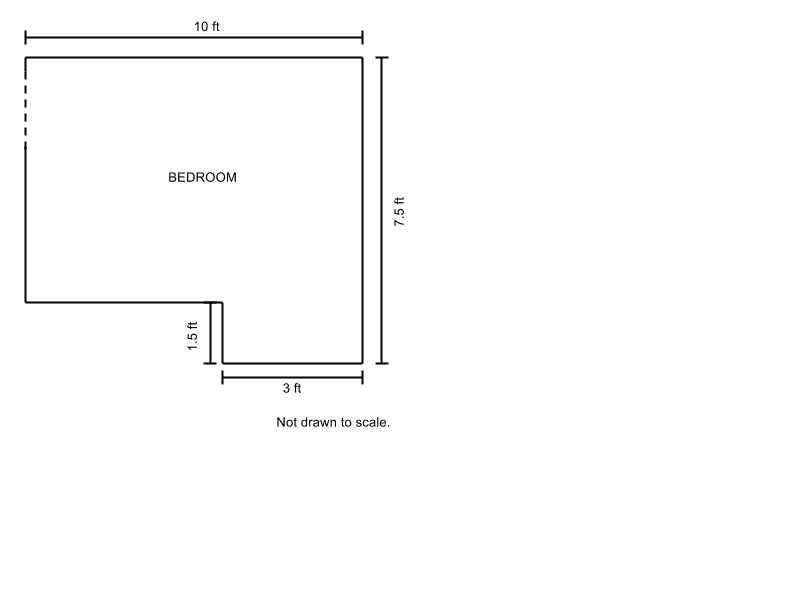
\includegraphics[scale=\shrinkfactor]{figures/ef03c3ec0a02a75ede44fd0e0c4c04a0f0aedc9d.png}

\paragraph{Ans} $\$$ [[? input-number 1]]  290.25

\paragraph{Hint 1}Sarah�s bedroom has two rectangular areas, large and small, to cover with carpet. Area of a rectangle is equal to its length times its width. 

The small rectangle is $\blue{3}\text{ ft}$ long and $\blue{1.5}\text{ ft}$ wide. The small rectangle has an area of: 

\begin{align*} A &= \blue{3}\cdot\blue{1.5}\\
&= \blue{4.5} \text{ sq ft}\end{align*}


\paragraph{Hint 2}The large rectangle is $\pink{10}\text{ ft}$ long and $(\pink{7.5 - 1.5})\text{ ft}$ wide. The large rectangle has an area of:

\begin{align*} A &=\pink{10}\cdot(\pink{7.5-1.5})\\&=\pink{10}\cdot\pink{6}\\
&= \pink{60} \text{ sq ft}\end{align*}


\paragraph{Hint 3}Let's find the total area of Sarah�s bedroom by adding the areas of the large and small rectangles together:

\begin{align*} A 
&= \blue{4.5} + \pink{60} \\
&= \purple{64.5} \text{ ft}^2\end{align*}

\paragraph{Hint 4}Sarah has $\purple{64.5}\text{ ft}^2$ to cover with carpet, and the cost of carpet is $\$\green{4.50}$ per square foot. Let's multiply the total area times the cost per area:

\begin{align*} &= \green{4.50}\cdot\purple{64.5}\\&=\$\red{290.25}\end{align*}

\paragraph{Hint 5}Sarah will pay $\$\red{290.25}$ to install wall-to-wall carpet in her bedroom.



\medskip
\noindent
\textbf{Tags:} {\footnotesize Images with English text,  Area, volume, and surface area of 2d and 3d objects, CC.7.G.B.6}\\
\textbf{Version:} 76730e30.. 2013-10-14
\smallskip\hrule





\section{\href{https://www.khanacademy.org/devadmin/content/items/xb0e4e814268fd586}{xb0e4e814268fd586}}

\noindent
The Ubas are moving from Houston to Egypt. They pack their belongings in rectangular crates and hire a boxcar to ship the crates across land and sea.  The crates are made specifically to fit inside the boxcar with their bases facing down. Each crate has a base $5\text{ m}$ long by $1.5\text{ m}$ wide and height $2\text{ m}$. The boxcar is $15\text{ m}$ long, $3\text{ m}$ wide and $4\text{ m}$ high. 

**How many crates can The Ubas fit into one boxcar?**


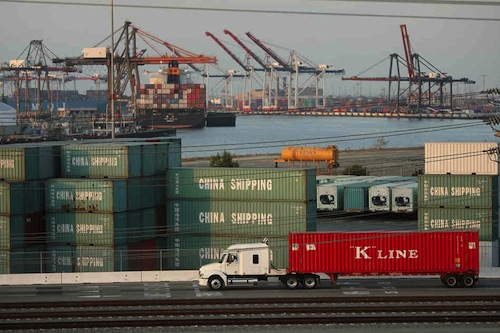
\includegraphics[scale=\shrinkfactor]{figures/203f27adba8bd870f05dc901ffbda2840eaf7d90.jpeg}

\paragraph{Ans} [[? input-number 1]] crates  12

\paragraph{Hint 1}Let's find the relationship between the lengths, widths and heights of the crate and boxcar:

\begin{align*} 5\text{ m}\times3&=15\text{ m}\\\\1.5\text{ m}\times2&=3\text{ m}\\\\2\text{ m}\times2&=4\text{ m}\end{align*}

\paragraph{Hint 2}Because the dimensions of the crate and boxcar are related, we can relate the volumes of the crate and boxcar in cubic meters. If we divide the volume of the boxcar by the volume of a crate, we can find how many crates The Ubas can fit into one boxcar.

The formula for volume $V$ of a rectangular prism is:

$\text{V} = \text{length}\cdot\text{width}\cdot\text{height}$

\paragraph{Hint 3}Let's find  $V$ of the boxcar in cubic meters:

\begin{align*} \text{V} &= \text{length}\cdot\text{width}\cdot\text{height}\\&=15\times3\times4\\&=\blue{180}\text{ m}^3\end{align*}

\paragraph{Hint 4}Let's find  $V$ of a crate in cubic meters:

\begin{align*} \text{V} &= \text{length}\cdot\text{width}\cdot\text{height}\\&=5\times1.5\times2\\&=\pink{15}\text{ m}^3\end{align*}

\paragraph{Hint 5}Now, let's divide the volume of the boxcar by the volume of a crate to find how many crates:

\begin{align*}\ &=\blue{180}\div\pink{15}\\&=\green{12}\end{align*}

\paragraph{Hint 6}The Ubas can fit $\green{12}$ crates into one boxcar.



\medskip
\noindent
\textbf{Tags:} {\footnotesize Image needs attribution,  Area, volume, and surface area of 2d and 3d objects, CC.7.G.B.6}\\
\textbf{Version:} 37895a06.. 2013-10-14
\smallskip\hrule





\section{\href{https://www.khanacademy.org/devadmin/content/items/xb2ab1d8c26fd802e}{xb2ab1d8c26fd802e}}

\noindent
Matt is making a crazy math construction. He wants to create $360$ small pyramids out of paper he folds, then glue together identical sides until he makes a large pyramid. One small pyramid contains a square base with side lengths $a$ and $4$ equilateral triangles with base $a$ and height $h$. The height $h$ is $3\text{ cm}$. The length $a$ is  $3.5\text{ cm}$. 

**In square centimeters what is the minimum amount of paper Matt needs to create $360$ small pyramids? (Assume there is no wasted paper.)**


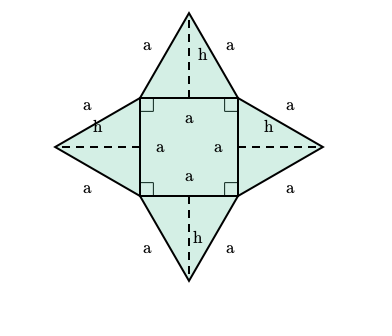
\includegraphics[scale=\shrinkfactor]{figures/6c9db7e28a2e7a3f87f8691e8eff1b044f8acbfd.png}

\paragraph{Ans} [[? input-number 1]] $\text{cm}^2$  11970

\paragraph{Hint 1}Let�s determine the surface area (SA) of one small pyramid in square centimeters. Then, we can multiply the surface area of one small pyramid times $\gray{360}$ to find how many square centimeters of paper Matt needs.

\paragraph{Hint 2}Let�s find the total surface area of a small pyramaid by finding the surface areas of $1$ square and $\purple4$ triangles.

 Area of a square is equal to its length squared. There is $1$ square side with side lengths $\blue{3.5}\text{ cm}$:
 
\begin{align*} SA &= \blue{3.5}^2\\
&= 12.25\text{ cm}^2\end{align*}

Area of a triangle is equal to one half its base times its height $h$. There are $\purple4$ triangles with a base of $\blue{3.5}$ and height of $\pink{3}\text{ cm}$:
 
\begin{align*} SA &= \purple{4}\times\dfrac{1}{2}\times\blue{3.5}\times\pink{3}\\
&= 21\text{ cm}^2\end{align*}

Let�s sum together all the surface areas to find the total surface area of one box: 

\begin{align*} SA &=12.25 + 21\\
&=  33.25\text{ cm}^2\end{align*}

\paragraph{Hint 3}Let's multiply the total area by $\gray{360}$ to find the amount of paper Matt needs:

\begin{align*} SA &= \gray{360}\times33.25\\&= \red{11970}\text{ cm}^2\end{align*}

\paragraph{Hint 4}Matt needs a minimum of $\red{11970}\text{ cm}^2$ of paper to create $\gray{360}$ small pyramids.



\medskip
\noindent
\textbf{Tags:} {\footnotesize Image needs attribution,  Area, volume, and surface area of 2d and 3d objects, CC.7.G.B.6}\\
\textbf{Version:} 29f350c3.. 2013-10-14
\smallskip\hrule





\section{\href{https://www.khanacademy.org/devadmin/content/items/xbab0d531f221f744}{xbab0d531f221f744}}

\noindent
A crew is excavating a construction site to build a new swimming pool. The crew fills the box of a dump truck to the top with dirt. The box is $16\text{ m}$ long, $3\text{ m}$ wide, and $8\text{ m}$ high. In transport to the dump site, the volume of the soil decreases $20\%$ as it settles in the box. 

**What is the height in feet of the dirt at the dump site?**



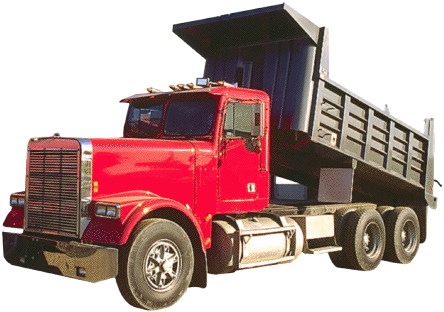
\includegraphics[scale=\shrinkfactor]{figures/e5db961622b94a55a7cbe0a2b2c1a6c7_AdPanel.png}

\paragraph{Ans} [[? input-number 1]] $\text{m}$  6.4

\paragraph{Hint 1}The length and width of the soil in the box does not change, but the height does change. Only the height of the soil decreases $20\%$. So, the soil is $\green{80}\%$ of its original height.



\paragraph{Hint 2}Let's multiply the height $\purple{8}\text{ m}$ by $\green{0.8}$  to find the height of the soil at the dump site:

\begin{align*} h &= \green{0.8}\cdot\purple{8}\\&= \pink{6.4}\text{ m}\end{align*}

\paragraph{Hint 3}The soil is $\pink{6.4}\text{ m}$ at the dump site.



\medskip
\noindent
\textbf{Tags:} {\footnotesize Image needs attribution,  Area, volume, and surface area of 2d and 3d objects, CC.7.G.B.6}\\
\textbf{Version:} 256e2635.. 2013-10-14
\smallskip\hrule





\section{\href{https://www.khanacademy.org/devadmin/content/items/xc3f3208be4a5eaec}{xc3f3208be4a5eaec}}

\noindent
A crew is excavating a construction site to build a new swimming pool. The crew fills the box of a dump truck to the top with dirt. The box is $45\text{ ft}$ long, $20\text{ ft}$ wide, and $23\text{ ft}$ high. In transport to the dump site, the volume of the soil decreases $10\%$ as it settles in the box.

**What is the volume of the dirt at the dump site in cubic feet?**




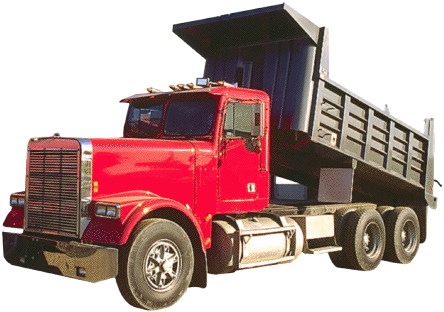
\includegraphics[scale=\shrinkfactor]{figures/e5db961622b94a55a7cbe0a2b2c1a6c7_AdPanel.png}

\paragraph{Ans} [[? input-number 1]] $\text{ft}^3$  18630

\paragraph{Hint 1}The length and width of the soil in the box does not change, but the height does change. Only the height of the soil decreases $10\%$. 

In other words, the soil is $\green{90}\%$ of its original height at the dump site, since $100\%-10\%=\green{90}\%$.



\paragraph{Hint 2}Let's multiply the original height $\purple{23}\text{ ft}$ by $\green{0.9}$  to find the height of the soil at the dump site:

\begin{align*} h &= \green{0.9}\cdot\purple{23}\\&= \pink{20.7}\text{ ft}\end{align*}

\paragraph{Hint 3}Now, let's find the volume of the box using the formula for volume $\text{V}$ of a rectangular prism and the dimensions of the soil at the dump site:

\begin{align*} \text{V} &= \text{length}\cdot\text{width}\cdot\text{height}\\
&= 45\cdot20\cdot\pink{20.7}\\
&= \blue{18630}\text{ ft}^3\end{align*}

\paragraph{Hint 4}The volume of the dirt at the dump site is $\blue{18630}\text{ ft}^3$.



\medskip
\noindent
\textbf{Tags:} {\footnotesize Image needs attribution,  Area, volume, and surface area of 2d and 3d objects, CC.7.G.B.6}\\
\textbf{Version:} 80bf6c9f.. 2013-10-14
\smallskip\hrule





\section{\href{https://www.khanacademy.org/devadmin/content/items/xd0f91d87d96a4556}{xd0f91d87d96a4556}}

\noindent
The company Digit Tech designs a new SmartPhone. The packaging includes an open box made out of cardboard. The dimensions of the box are $12\text{ cm}$ long, $9\text{ cm}$  wide and $9\text{ cm}$  high. Digit Tech expects to sell $1500$ phones and package each phone individually in a box. 

**In square centimeters what is the minimum amount of cardboard Digit Tech needs to package all $1500$ new SmartPhones? (Assume there is no wasted cardboard.)**
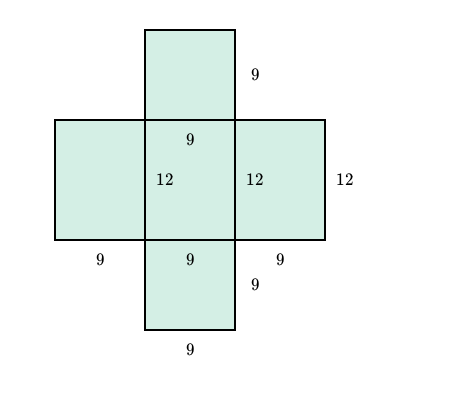
\includegraphics[scale=\shrinkfactor]{figures/58c6efd13e5e01bbbebe92786bfe9b15789a0fe9.png}

\paragraph{Ans} [[? input-number 1]] $\text{cm}^2$  729000

\paragraph{Hint 1}Let�s determine the surface area (SA) of one box in square centimeters. Then, we can multiply the surface area of one box times $\purple{1500}$ to find how many square centimeters of cardboard are needed.

The box has $5$ sides: $1$ bottom and $2$ sets of equal sides opposite each other.

\paragraph{Hint 2}Let�s find the total surface area of the box. Area of a rectangle is equal to its length times its width. Let's find the surface areas of the $5$ rectangular sides.

There are $\gray{2}$ sides $\blue{12}\text{ cm}$ long and $\green{9}\text{ cm}$ high:
 
\begin{align*} SA &= \gray{2}\times\blue{12}\times\green{9}\\
&= 216\text{ cm}^2\end{align*}

There are $\gray{2}$ sides $\pink{9}\text{ cm}$ wide and $\green{9}\text{ cm}$ high:
 
\begin{align*} SA &= \gray{2}\times\pink{9}\times\green{9}\\
&= 162\text{ cm}^2\end{align*}

There is $\gray{1}$ side (the bottom) $\blue{12}$ cm long and $\pink{9}$ cm wide:

\begin{align*} SA &= \gray{1}\times\blue{12}\times\pink{9}\\
&= 108\text{ cm}^2\end{align*}

Let�s sum together all the surface areas to find the total surface area of one box: 

\begin{align*} SA &= 216 + 162 + 108\\
&= 486\text{ cm}^2\end{align*}

\paragraph{Hint 3}Let's multiply the total area by $\purple{1500}$ boxes to find the amount of cardboard:

\begin{align*} SA &= \purple{1500}\times486\\&= \pink{729000}\text{ cm}^2\end{align*}

\paragraph{Hint 4}Digit Tech needs a minimum of $\pink{729,000}\text{ cm}^2$ of cardboard to package all $\purple{1500}$ new SmartPhones individually.



\medskip
\noindent
\textbf{Tags:} {\footnotesize Image needs attribution,  Area, volume, and surface area of 2d and 3d objects, CC.7.G.B.6}\\
\textbf{Version:} 6b330ffc.. 2013-10-14
\smallskip\hrule





\section{\href{https://www.khanacademy.org/devadmin/content/items/xd27f560044011f21}{xd27f560044011f21}}

\noindent
Abby plans to put in wall-to-wall carpet in her bedroom. She measures the dimensions of her bedroom and sketches up the following floor plan.  The carpet costs $\$9.50$ per square meter. 

**How much will Abby pay for wall-to-wall carpet for her bedroom?**

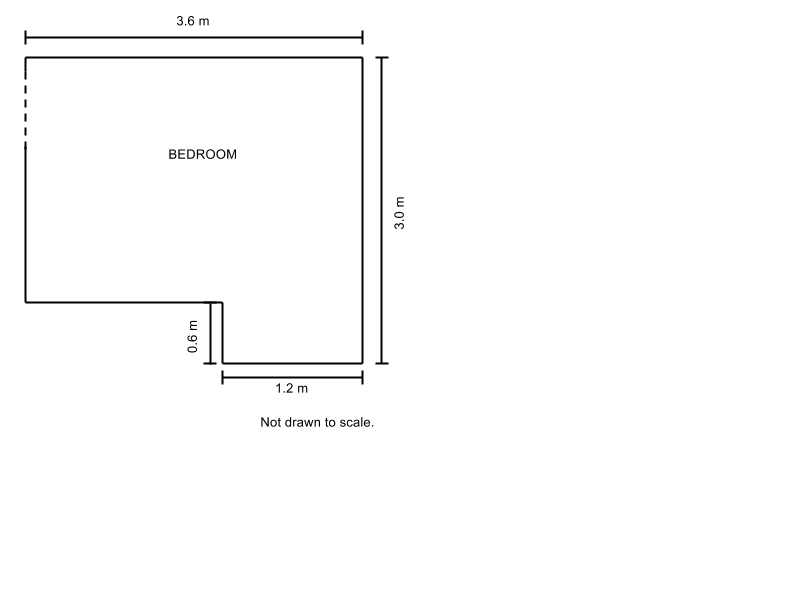
\includegraphics[scale=\shrinkfactor]{figures/4b8b055546ab1cc405a81ad93726d4dc5e88bf23.png}

\paragraph{Ans} $\$$ [[? input-number 1]]  88.92

\paragraph{Hint 1}Abby�s bedroom has two rectangular areas, large and small, to cover with carpet. Area of a rectangle is equal to its length times its width. 

The small rectangle is $\blue{0.6}\text{ m}$ long and $\blue{1.2}\text{ m}$ wide. The small rectangle has an area of:  

\begin{align*} A &= \blue{0.6}\times\blue{1.2}\\
&= \blue{0.72} \text{ m}^2\end{align*}


\paragraph{Hint 2}The large rectangle is $\pink{3.6}\text{ m}$ long and $(\pink{3.0 - 0.6})\text{ m}$ wide. The large rectangle has an area of:

\begin{align*} A &=\pink{3.6}\times(\pink{3.0 - 0.6})\\&=\pink{3.6}\times\pink{2.4}\\
&= \pink{8.64} \text{ m}^2\end{align*}


\paragraph{Hint 3}Let's find the total area of Abby�s bedroom by adding the areas of the large and small rectangles together:

\begin{align*} A 
&= \blue{0.72} + \pink{8.64} \\
&= \purple{9.36} \text{ m}^2\end{align*}

\paragraph{Hint 4}Abby has $\purple{9.36}\text{ m}^2$ to cover with carpet, and the cost of carpet is $\$\green{9.50}$ per square foot. Let's multiply the total area times the cost per area:

\begin{align*} &= \green{9.50}\times\purple{9.36}\\&=\$\red{88.92}\end{align*}

\paragraph{Hint 5}Abby will pay $\$\red{88.92}$ to install wall-to-wall carpet in her bedroom.



\medskip
\noindent
\textbf{Tags:} {\footnotesize Images with English text,  Area, volume, and surface area of 2d and 3d objects, CC.7.G.B.6}\\
\textbf{Version:} 7e971689.. 2013-10-14
\smallskip\hrule





\section{\href{https://www.khanacademy.org/devadmin/content/items/xd6227f8ede3bdcf6}{xd6227f8ede3bdcf6}}

\noindent
Priya plans to put in wall-to-wall carpet in her bedroom. She measures the dimensions of her bedroom and sketches up the following floor plan. The carpet costs $\$3.75$ per square foot. 

**How much will Priya pay for wall-to-wall carpet for her bedroom?**

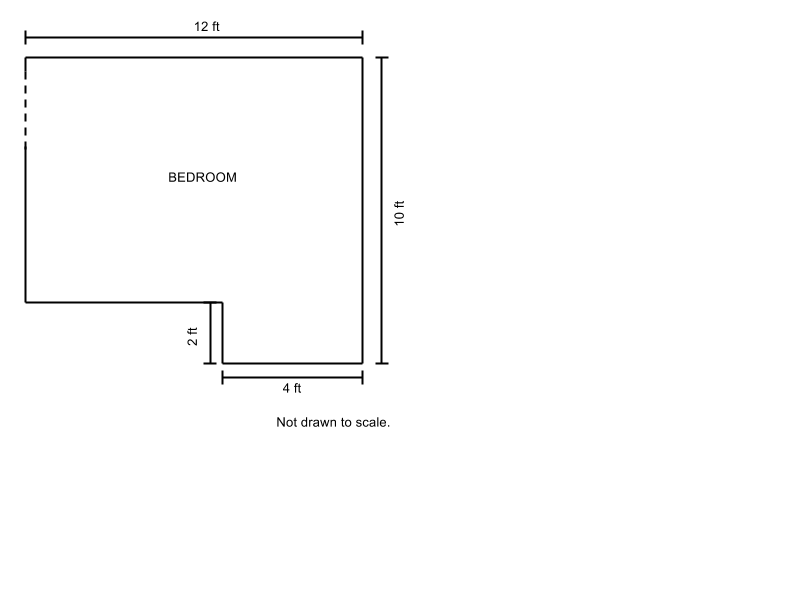
\includegraphics[scale=\shrinkfactor]{figures/e7e9250b0ae677c4df0624a0aed55e9862aefa00.png}

\paragraph{Ans} $\$$ [[? input-number 1]]  390

\paragraph{Hint 1}Priya�s bedroom has two rectangular areas, large and small, to cover with carpet. Area of a rectangle is equal to its length times its width. 

The small rectangle is $\blue{4}\text{ ft}$ long and $\blue{2}\text{ ft}$ wide. The small rectangle has an area of: 

\begin{align*} A &= \blue{4}\cdot\blue{2}\\
&= \blue{8} \text{ sq ft}\end{align*}


\paragraph{Hint 2}The large rectangle is $\pink{12}\text{ ft}$ long and $(\pink{10 - 2})\text{ ft}$ wide. The large rectangle has an area of:

\begin{align*} A &=\pink{12}\cdot(\pink{10-2})\\&=\pink{12}\cdot\pink{8}\\
&= \pink{96} \text{ sq ft}\end{align*}


\paragraph{Hint 3}Let's find the total area of Priya�s bedroom by adding the areas of the large and small rectangles together:

\begin{align*} A 
&= \blue{8} + \pink{96} \\
&= \purple{104} \text{ sq ft}\end{align*}

\paragraph{Hint 4}Priya has $\purple{104}\text{ sq ft}$ to cover with carpet, and the cost of carpet is $\$\green{3.75}$ per square foot. Let's multiply the total area times the cost per area:

\begin{align*} &= \green{3.75}\cdot\purple{104}\\&=\$\red{390}\end{align*}

\paragraph{Hint 5}Priya will pay $\$\red{390}$ to install wall-to-wall carpet in her bedroom.



\medskip
\noindent
\textbf{Tags:} {\footnotesize Images with English text,  Area, volume, and surface area of 2d and 3d objects, CC.7.G.B.6}\\
\textbf{Version:} d95c8310.. 2013-10-14
\smallskip\hrule





\section{\href{https://www.khanacademy.org/devadmin/content/items/xd9d03a194cdc8ae4}{xd9d03a194cdc8ae4}}

\noindent
Jamie wants to know the volume of her gold ring in cubic inches. She gets a rectangular glass with a base $3\text{ in}$ by $2\text{ in}$ and fills the glass $4 \text{ in}$ high with water. Jamie drops her gold ring in the glass and measures the new height of the water to be $4.25\text{ in}$. 

**What is the volume of Jamie's ring in cubic inches?**



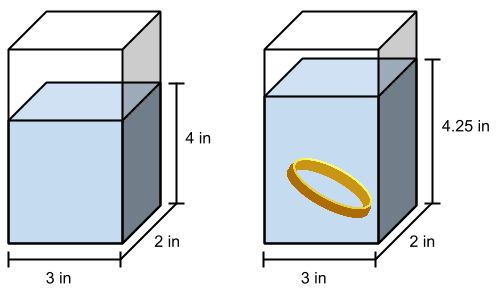
\includegraphics[scale=\shrinkfactor]{figures/516cc151bd5a4650508da70b542bb9239c2c171d.png}

\paragraph{Ans} [[? input-number 1]] $\text{in}^3$  1.5

\paragraph{Hint 1}The change in volume of the water is caused by adding the volume of Jamie's gold ring to the volume of the water. Let's find the change in volume to find the volume of the gold ring.

Volume $V$ of a rectangular prism can be calculated using the formula:

$\text{V} = \text{length}\cdot\text{width}\cdot\text{height}$

\paragraph{Hint 2}The length $\green3\text{ in}$ and width $\purple2\text{ in}$ of the water in the rectangular glass does not change, but the height does change. 

\paragraph{Hint 3}The change in height of the water is $\blue{(4.25-4)}\text{ in}$. Let's find $V$ of the change in water:

\begin{align*} \text{V} &= \text{length}\cdot\text{width}\cdot\text{height}\\
&= \green3\cdot\purple2\cdot\blue{(4.25-4)}\\&= \green3\cdot\purple2\cdot\blue{(0.25)}\\
&= \red{1.5}\text{ in}^3\end{align*}

\paragraph{Hint 4}The volume of Jamie's gold ring is $\red{1.5}\text{ in}^3$.



\medskip
\noindent
\textbf{Tags:} {\footnotesize Image needs attribution,  Area, volume, and surface area of 2d and 3d objects, CC.7.G.B.6}\\
\textbf{Version:} a2cf8da3.. 2013-10-14
\smallskip\hrule





\section{\href{https://www.khanacademy.org/devadmin/content/items/xe36af4fb7a84ecf5}{xe36af4fb7a84ecf5}}

\noindent
Meghan made each of her $10$ girlfriends a pair of earrings. To wrap the pairs individually, she creates a simple cardboard gift box to fold into a pyramid. The base is a square with side lengths $6\text{ in}$. The sides are $4$ equilateral triangles with side lengths $6\text{ in}$ and height $h$. The height $h$ is equal to $5\dfrac{1}{5}\text{ in}$. 

**In square inches what is the minimum amount of cardboard Meghan needs to create $10$ gift boxes to wrap each pair of earrings individually? (Assume there is no wasted cardboard.)**
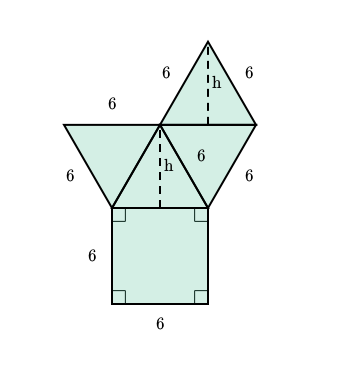
\includegraphics[scale=\shrinkfactor]{figures/b44301196b30b73ea0989191991e2217cad1852d.png} 

\paragraph{Ans} [[? input-number 1]] $\text{in}^2$  984

\paragraph{Hint 1}Let�s determine the surface area (SA) of one box in square inches. Then, we can multiply the surface area of one box times $\gray{10}$ to find how many square inches of cardboard are needed. 

Let's use fractions throughout our calculations to avoid any rounding errors.

\paragraph{Hint 2}Let�s find the total surface area of the box by finding the surface areas of $1$ square and $\purple4$ triangles.

 Area of a square is equal to its length squared. There is $1$ square side with side lengths $\blue{6}\text{ in}$:
 
\begin{align*} SA &= \blue{6}^2\\
&= 36\text{ in}^2\end{align*}

Area of a triangle is equal to one half its base times its height $h$. There are $\purple4$ triangles with a base of $\blue{6}\text{ in}$ and height of $\pink{5\dfrac{1}{5}}\text{ in}$:
 
\begin{align*} SA &= \purple{4}\times\dfrac{1}{2}\times\blue{6}\times\pink{5\dfrac{1}{5}}\\\\&=\purple{4}\times\blue{6}\times\dfrac{1}{2}\times\pink{\dfrac{26}{5}}\\\\
&= \dfrac{624}{10}\\\\&= 62.4\text{ in}^2\end{align*}

Let�s sum together all the surface areas to find the total surface area of one box: 

\begin{align*} SA &= 36 + 62.4\\
&=  98.4\text{ in}^2\end{align*}

\paragraph{Hint 3}Let's multiply the total area by $\gray{10}$ boxes to find the amount of cardboard:

\begin{align*} SA &= \gray{10}\times 98.4\\&= \red{984}\text{ in}^2\end{align*}

\paragraph{Hint 4}Meghan needs a minimum of $\red{984}\text{ in}^2$ of cardboard to package all $\gray{10}$ pairs of earrings individually.



\medskip
\noindent
\textbf{Tags:} {\footnotesize Image needs attribution,  Area, volume, and surface area of 2d and 3d objects, CC.7.G.B.6}\\
\textbf{Version:} 274aea9a.. 2013-10-14
\smallskip\hrule





\section{\href{https://www.khanacademy.org/devadmin/content/items/xec1dd6aec52f6d8f}{xec1dd6aec52f6d8f}}

\noindent
Samuel plans to put in wall-to-wall carpet in his living room. He measures the edges of his living room and sketches up the following floor plan. The carpet costs $\$10$ per square foot. 

**How much will Samuel pay for wall-to-wall carpet for his living room?**
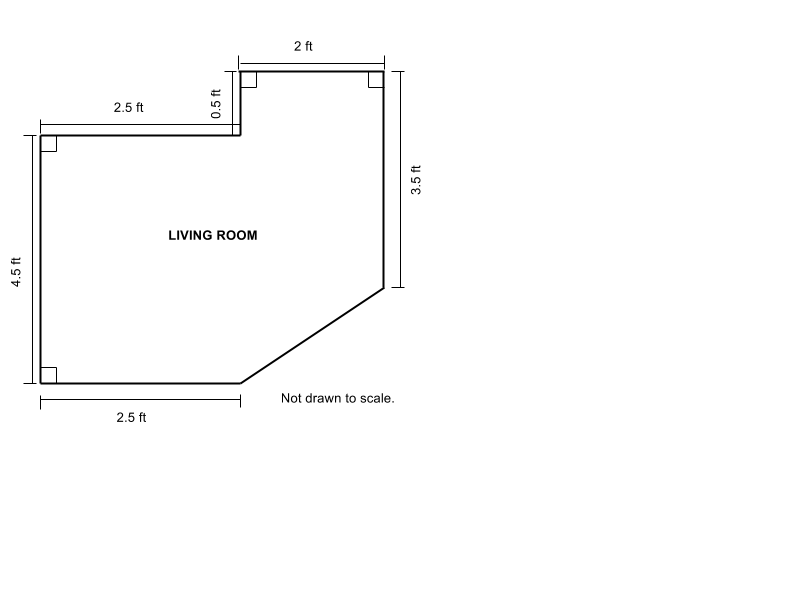
\includegraphics[scale=\shrinkfactor]{figures/53d9c248bb713a2335fbda13af0b0356b269f2e0.png}

\paragraph{Ans} $\$$ [[? input-number 1]]  197.5

\paragraph{Hint 1}Samuel's living room has $3$ rectangular areas and $1$ triangular area to cover with carpet. Let's find the total area of the living room floor in square feet to find how much carpet Samuel needs.

Area of a rectangle is equal to its length times its width. Area of a triangle is equal to one half its base times its height. 

\paragraph{Hint 2}From the vertical dimensions, we can determine the height of the triangle as $\red{1.5}\text{ ft}$. We can also find the dimensions of the areas. 
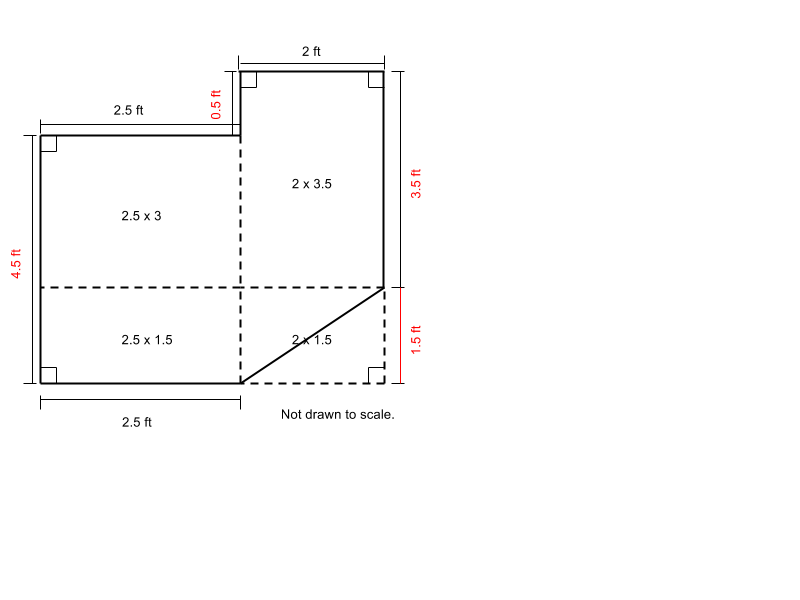
\includegraphics[scale=\shrinkfactor]{figures/a8949d21aeb173c5509f4ebf9685fc2f10ad38e0.png}

\paragraph{Hint 3}Let's find the total area of the living room by adding the areas of the $3$ rectangles and $1$ triangle together. 

\begin{align*}  
&= 2.5\times3 +2\times3.5+2.5\times1.5+ 0.5\times2\times\red{1.5}\\\\&=7.5+7+3.75+1.5\\\\
&= \purple{19.75} \text{ ft}^2\end{align*}

\paragraph{Hint 4}Samuel has $\purple{19.75}\text{ ft}^2$ to cover with carpet, and the cost of carpet is $\$\green{10}$ per square foot. Let's multiply the total area times the cost per area:

\begin{align*} &= \green{10}\times\purple{19.75}\\&=\$\blue{ 197.50}\end{align*}

\paragraph{Hint 5}Samuel will pay $\$\blue{197.50}$ to install wall-to-wall carpet in his living room.



\medskip
\noindent
\textbf{Tags:} {\footnotesize Images with English text,  Area, volume, and surface area of 2d and 3d objects, CC.7.G.B.6}\\
\textbf{Version:} c9bed14b.. 2013-10-14
\smallskip\hrule





\section{\href{https://www.khanacademy.org/devadmin/content/items/xef699039b85ac16e}{xef699039b85ac16e}}

\noindent
Phung plans to put in square tile flooring in his kitchen. The square tile has an $8$ inch side length. He measures the dimensions of his kitchen and sketches up the following floor plan. 

**How many tiles does Phung need to cover the entire area of his kitchen floor?**

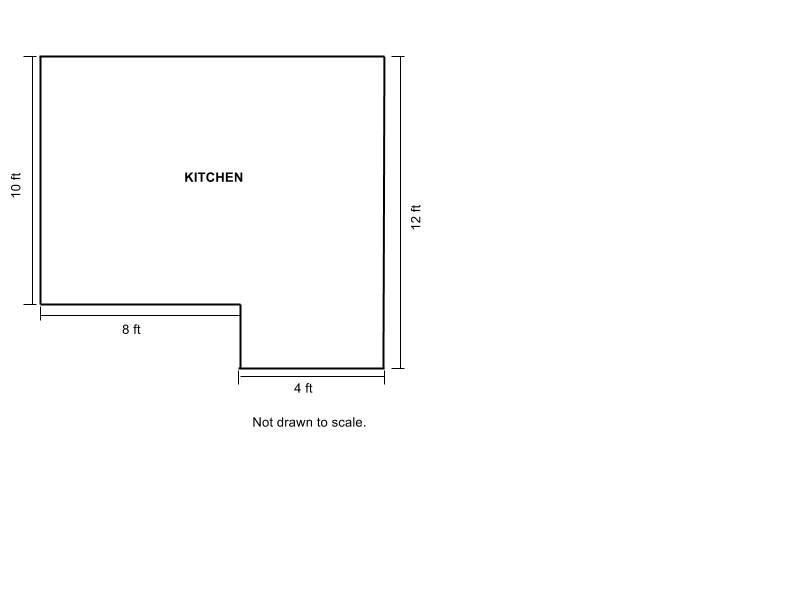
\includegraphics[scale=\shrinkfactor]{figures/319f9abe99981020ba1c629b71a38c8e2707617b.png}

\paragraph{Ans} [[? input-number 1]] tiles  288

\paragraph{Hint 1}Phung's kitchen has $2$ rectangular areas to cover with tiles. Let's find the total area of the kitchen floor in square feet, then divide by the area of one square tile to find how many tiles Phung needs.

\paragraph{Hint 2}Let's choose $2$ rectangular areas that will fit the $\blue8 \text{ in}$ square tiles.

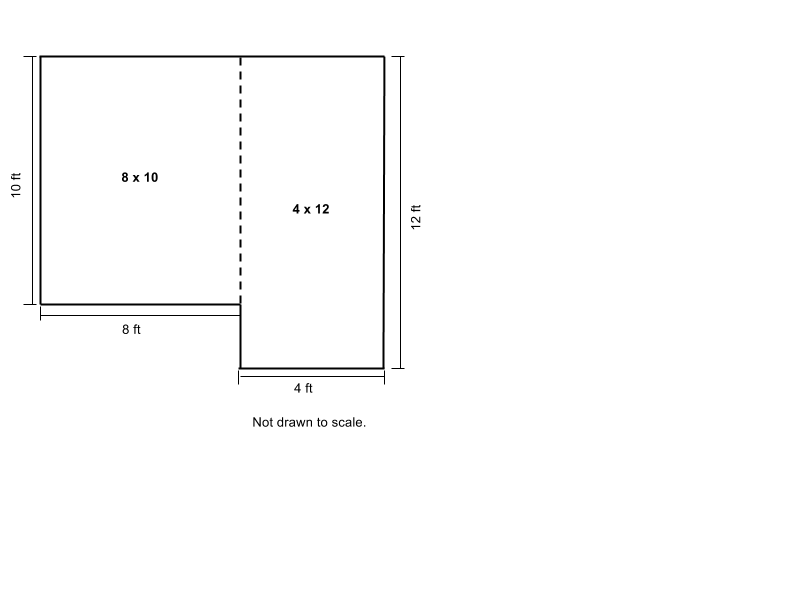
\includegraphics[scale=\shrinkfactor]{figures/d938baba62c24ee37bd6c943a1b53d74021beec3.png}

\paragraph{Hint 3}Now we can find the total area of the kitchen by adding the areas of the rectangles together. Area of a rectangle is equal to its length times its width. 

\begin{align*}  
&= 8\times10+4\times12\\[2mm]
&=80+48\\[2mm]
&= \purple{128} \text{ ft}^2
\end{align*}

The kitchen floor is $\purple{128}$ ft$^2$.

\paragraph{Hint 4}In feet each tile is a square with side length $\dfrac{\blue{8}}{12}$ ft.

The area of one tile is $\left(\dfrac{\blue{8}}{12}\right)^2=\green{\dfrac{64}{144}}$ ft$^2$. 

Let's divide the area of the kitchen floor by the area of one tile:

\begin{align*}&= \purple{128}\div\green{\dfrac{64}{144}}\\\\&= \purple{128}\times\green{\dfrac{144}{64}}\\\\&=\pink{288}\end{align*}

\paragraph{Hint 5}Phung needs $\pink{288}$ tiles to cover the entire area of his kitchen floor.



\medskip
\noindent
\textbf{Tags:} {\footnotesize CC.7.G.B.6}\\
\textbf{Version:} e7c55566.. 2013-10-18
\smallskip\hrule





\section{\href{https://www.khanacademy.org/devadmin/content/items/xfe7abf43d5f7336a}{xfe7abf43d5f7336a}}

\noindent
The Connors are moving from Boston to Iceland. They pack their belongings in rectangular crates and hire a boxcar to ship the crates across land and sea.  The crates are made specifically to fit inside the boxcar with their bases facing down. Each crate has a base $4\text{ m}$ long by $2\text{ m}$ wide and height $2.5\text{ m}$. The boxcar is $16\text{ m}$ long, $4\text{ m}$ wide and $5\text{ m}$ high. 

**How many crates can The Connors fit into one boxcar?**


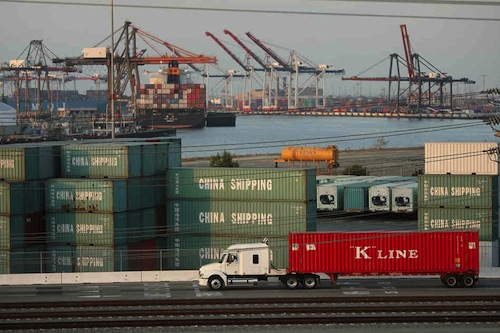
\includegraphics[scale=\shrinkfactor]{figures/203f27adba8bd870f05dc901ffbda2840eaf7d90.jpeg}

\paragraph{Ans} [[? input-number 1]] crates  16

\paragraph{Hint 1}Let's find the relationship between the lengths, widths and heights of the crate and boxcar:

\begin{align*} 4\text{ m}\times3&=16\text{ m}\\\\2\text{ m}\times2&=4\text{ m}\\\\2.5\text{ m}\times2&=5\text{ m}\end{align*}

\paragraph{Hint 2}Because the dimensions of the crate and boxcar are related, we can relate the volumes of the crate and boxcar in cubic meters. If we divide the volume of the boxcar by the volume of a crate, we can find how many crates The Connors can fit into one boxcar.

The formula for volume $V$ of a rectangular prism is:

$\text{V} = \text{length}\cdot\text{width}\cdot\text{height}$

\paragraph{Hint 3}Let's find  $V$ of the boxcar in cubic meters:

\begin{align*} \text{V} &= \text{length}\cdot\text{width}\cdot\text{height}\\&=16\times4\times5\\&=\blue{320}\text{ m}^3\end{align*}

\paragraph{Hint 4}Let's find  $V$ of a crate in cubic meters:

\begin{align*} \text{V} &= \text{length}\cdot\text{width}\cdot\text{height}\\&=4\times2\times2.5\\&=\pink{20}\text{ m}^3\end{align*}

\paragraph{Hint 5}Now, let's divide the volume of the boxcar by the volume of a crate to find how many crates:

\begin{align*}\ &=\blue{320}\div\pink{20}\\&=\green{16}\end{align*}

\paragraph{Hint 6}The Connors can fit $\green{16}$ crates into one boxcar. 



\medskip
\noindent
\textbf{Tags:} {\footnotesize Image needs attribution,  Area, volume, and surface area of 2d and 3d objects, CC.7.G.B.6}\\
\textbf{Version:} d0da3fa3.. 2013-10-14
\smallskip\hrule



%%  Create a directory called 'figures' in latex dir and run the following command 
%  wget -N \
%    https://ka-perseus-images.s3.amazonaws.com/203f27adba8bd870f05dc901ffbda2840eaf7d90.jpeg \
%    https://ka-perseus-images.s3.amazonaws.com/9b1e5c4a0a1124465ed46125df08ae907b12b004.png \
%    https://ka-perseus-images.s3.amazonaws.com/58a4ba6e006a4cfc3f99cbaea0652a702b968dff.png \
%    https://ka-perseus-images.s3.amazonaws.com/046f049679d81a6e9e292791541c4b03dbcf7768.png \
%    https://ka-perseus-images.s3.amazonaws.com/bf7eaf5031a5e491d306dade1ef1176bfc6d4857.png \
%    https://ka-perseus-graphie.s3.amazonaws.com/9ee87af5745eecf3946aa60a923f2788c1dea2bf.png \
%    https://ka-perseus-images.s3.amazonaws.com/6a170f3839757fae9ea33580d7e13567cc0e63e8.png \
%    https://ka-perseus-graphie.s3.amazonaws.com/a118c7f7a06b93f92f4dfa5551cf739f2755885d.png \
%    http://www.farmersagent.com/Assets/Agents/tbrown8/Images/e5db961622b94a55a7cbe0a2b2c1a6c7_AdPanel.png \
%    https://ka-perseus-graphie.s3.amazonaws.com/69a70b16cec3997bfa665a611382451946b7bf54.png \
%    https://ka-perseus-graphie.s3.amazonaws.com/9b1a8c58e358c5d122dd18071886f4cdf8867b8f.png \
%    https://ka-perseus-images.s3.amazonaws.com/3acac9e0deb063daeeca4749bfd6c9dbd2289ce2.png \
%    https://ka-perseus-images.s3.amazonaws.com/809320a51fcfe278f60fb9dff4257df10294d43d.png \
%    https://ka-perseus-graphie.s3.amazonaws.com/6c9db7e28a2e7a3f87f8691e8eff1b044f8acbfd.png \
%    https://ka-perseus-images.s3.amazonaws.com/4b9d2e0994214f17fec92b441910951b128b26b4.png \
%    https://ka-perseus-images.s3.amazonaws.com/ef03c3ec0a02a75ede44fd0e0c4c04a0f0aedc9d.png \
%    https://ka-perseus-graphie.s3.amazonaws.com/58c6efd13e5e01bbbebe92786bfe9b15789a0fe9.png \
%    https://ka-perseus-images.s3.amazonaws.com/4b8b055546ab1cc405a81ad93726d4dc5e88bf23.png \
%    https://ka-perseus-images.s3.amazonaws.com/e7e9250b0ae677c4df0624a0aed55e9862aefa00.png \
%    https://ka-perseus-images.s3.amazonaws.com/516cc151bd5a4650508da70b542bb9239c2c171d.png \
%    https://ka-perseus-graphie.s3.amazonaws.com/b44301196b30b73ea0989191991e2217cad1852d.png \
%    https://ka-perseus-images.s3.amazonaws.com/53d9c248bb713a2335fbda13af0b0356b269f2e0.png \
%    https://ka-perseus-images.s3.amazonaws.com/a8949d21aeb173c5509f4ebf9685fc2f10ad38e0.png \
%    https://ka-perseus-images.s3.amazonaws.com/319f9abe99981020ba1c629b71a38c8e2707617b.png \
%    https://ka-perseus-images.s3.amazonaws.com/d938baba62c24ee37bd6c943a1b53d74021beec3.png \


\end{document}

